\noindent In this section, we decided to describe the most significant implementation details and quote code fragments of our project with brief explanation. Finally, we noticed how we tested our software.

\subsection{Significant Implementation Details}
\noindent After several months of unremitting efforts, various methods have been tried. From scratch, we implemented several key functions of the original design step by step, and based on this, we have continuously improved and added some additional functions. We introduce them separately for the web client and the iOS mobile client.
\subsubsection{Desktop Client}
\noindent User login Interface Introduction:
\begin{itemize}
    \item \textbf{Registration Functions}: When registering in this web page, users only need to provide user-defined user name and password, and the system will automatically assign a UID to them. In the background system operation, the system background system will automatically distinguish different users according to their UID. The final interface of registration function is shown in Fig.\ref{register}.
    
    \begin{figure}[H]
     \centering
     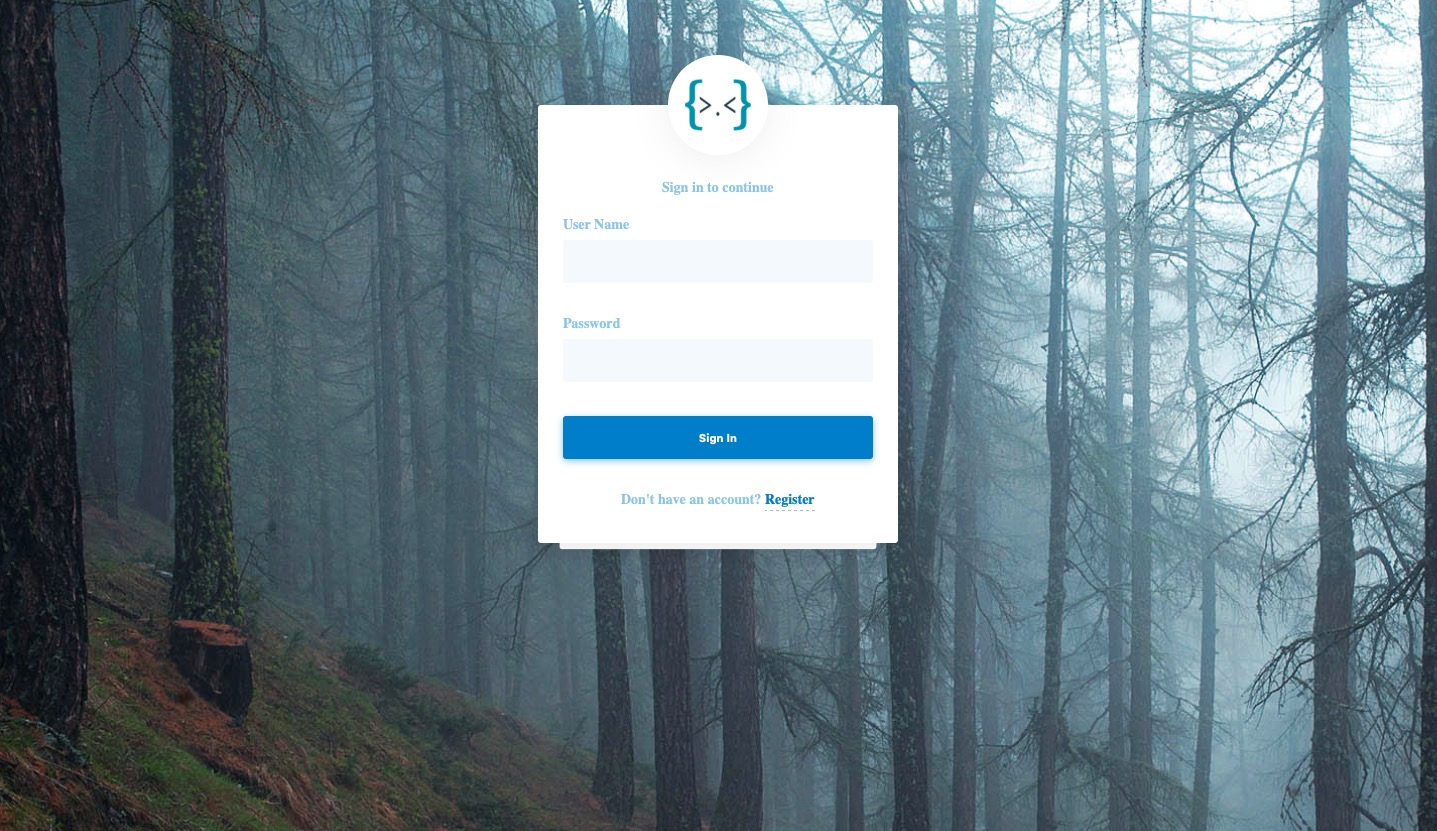
\includegraphics[width=.8\textwidth]{signinui.jpeg} 
     \caption{Registration Interface}
     \label{register}
    %  \vspace{-1em}
     \end{figure}
    
    \item \textbf{Login Interface Functions}: In the process of implementing the login function, we extra use the channel encryption method to encrypt the user password. To be specific, we use the hash algorithm to ensure the security of the user. Because the hash function is unidirectional, once the user name and password are provided when the user registers, the system automatically assigns the UID background to distinguish the user according to the UID. The final interface of login function is shown in Fig.\ref{login}.
    
      \begin{figure}[H]
     \centering
     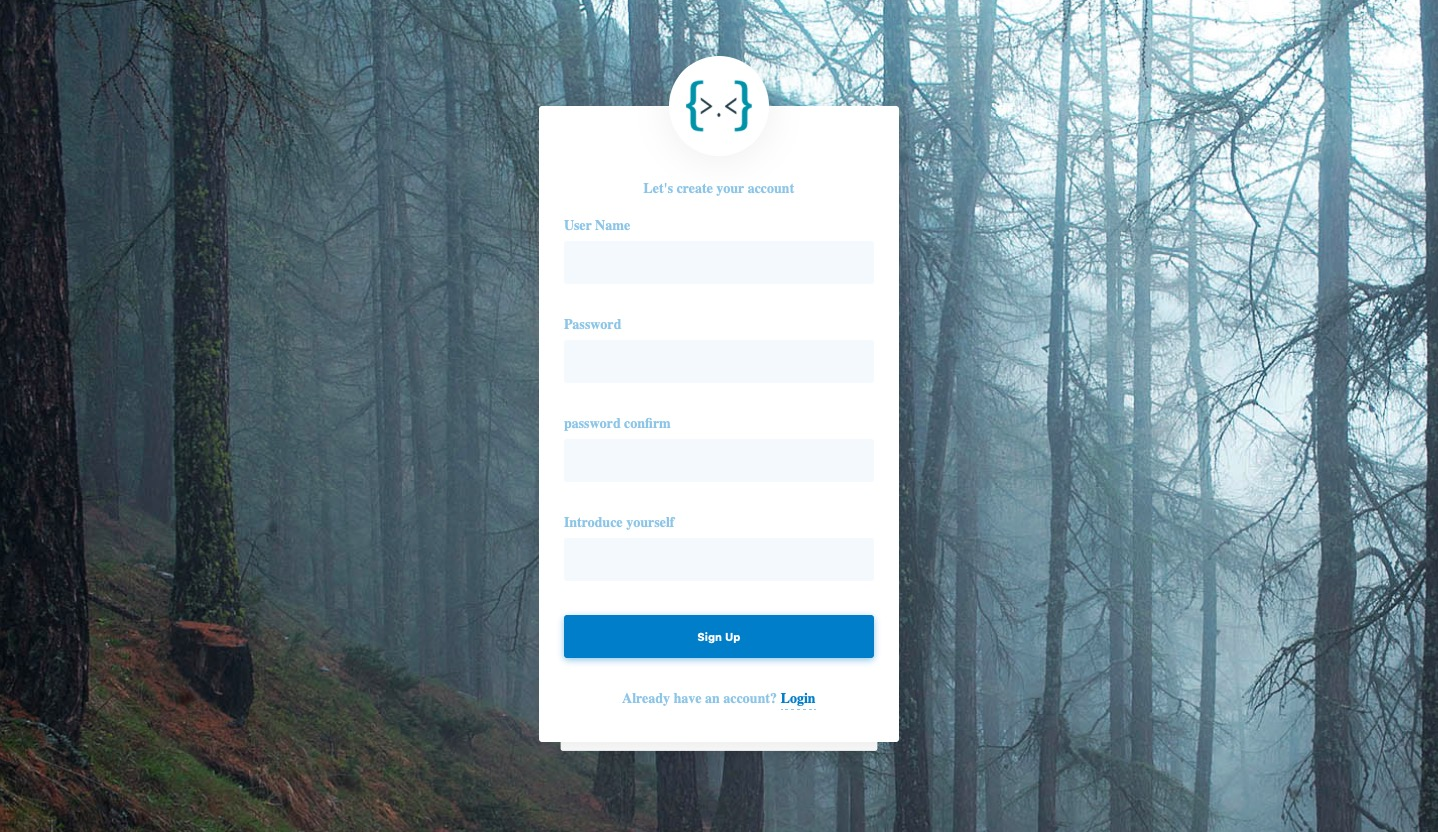
\includegraphics[width=.8\textwidth]{loginui.jpeg}
     \caption{Login Interface}
     \label{login}
     \vspace{-1em}
     \end{figure}
     
     \item \textbf{Password Changing Interface Functions}: In this page, users can change their password and finally login to the system by using their new password. The final interface of changing the password is shown in Fig.\ref{change}.
      
      \begin{figure}[H]
     \centering
     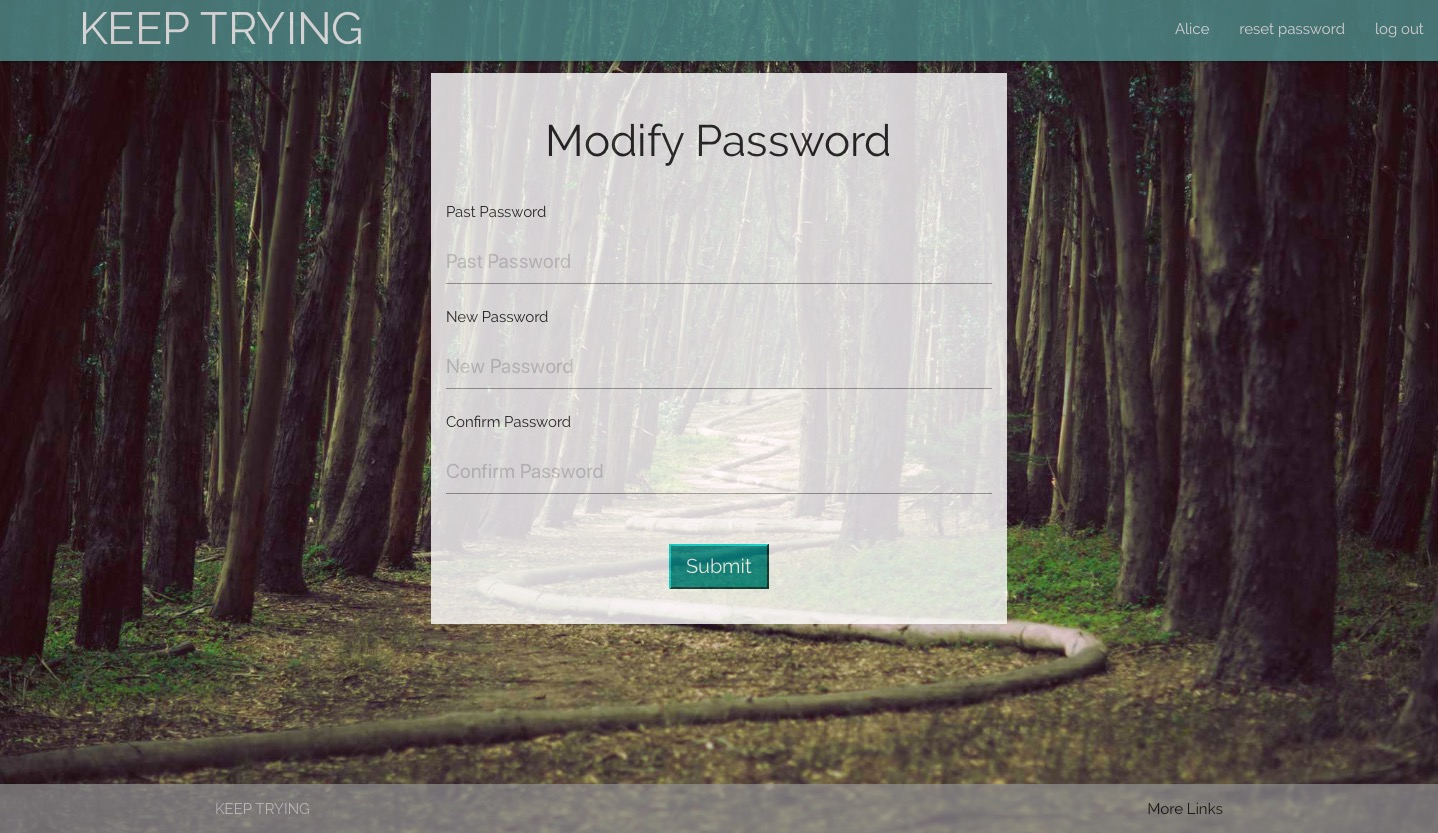
\includegraphics[width=.8\textwidth]{changepasswdui.jpeg}
     \caption{Password Changing Interface}
     \label{change}
     \end{figure}
     
    
\end{itemize}


\noindent Homepage function introduction:
\begin{itemize}
     \item \textbf{User Detail}: This module shows the user's details, including the user name, creation time and a simple slogan.
     \item \textbf{Error News}: This module shows all conflicting files, including the id of the file, the reason of the error, and the last update time of the file.
     \item \textbf{Your Files}: In this module users can manage their own files, including the existing file id, name, creator and last update time. In addition, users can also create new files via the \texxx{create\_new\_file} button, or select a document upload from the local storage.

\end{itemize}



\noindent The final interface of Homepage is shown in Fig.\ref{home}.
    \begin{figure}[H]
     \centering
     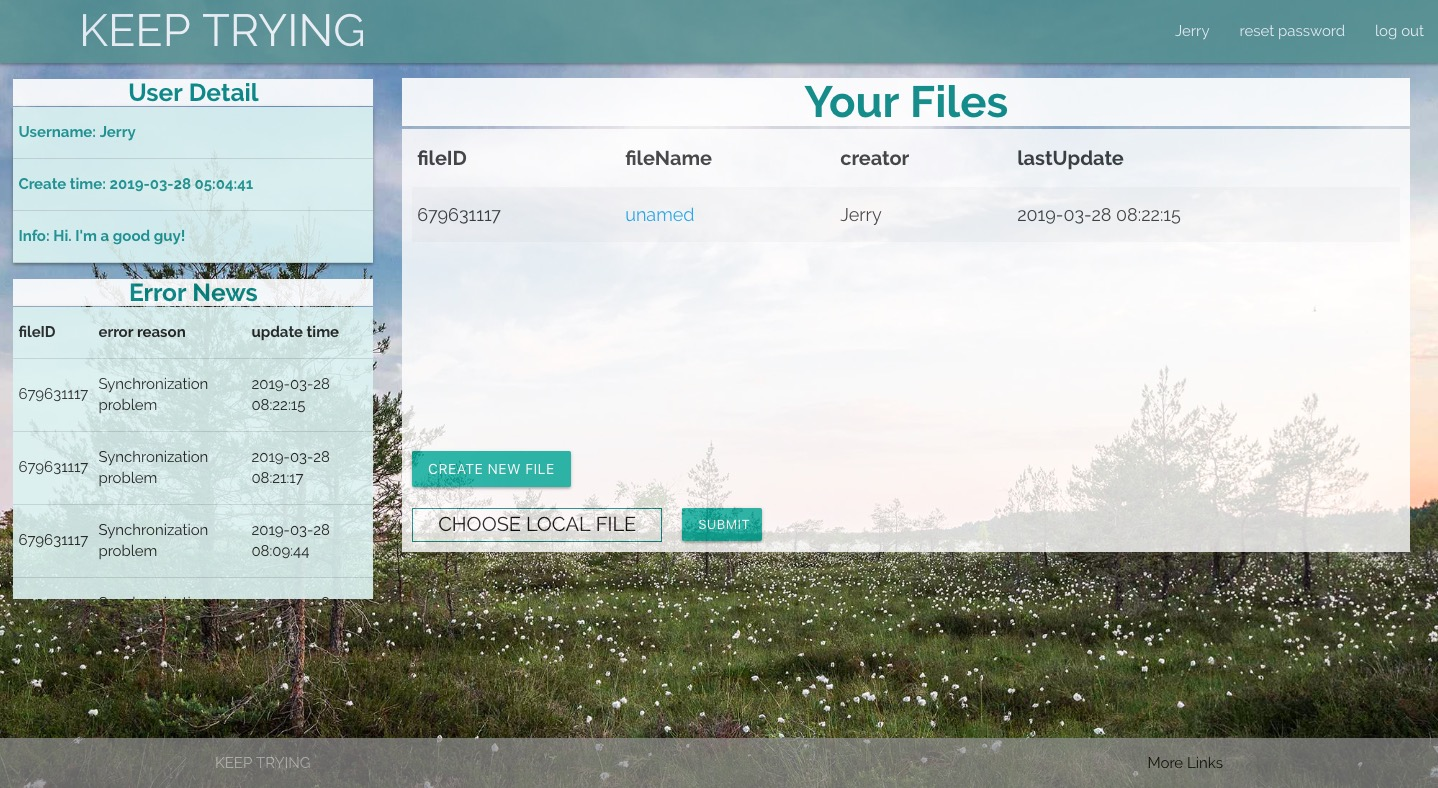
\includegraphics[width=.8\textwidth]{homep.jpeg}
     \caption{Homepage}
     \label{home}
     \end{figure}
    



\noindent Edit page functions introduction
\begin{itemize}
    \item \textbf{Content modification}: This module contains file content modification and the filename modification.
   \item \textbf{File Information}: You can see the file information in this module, including the file name, the creator of the file, the time of the last modification, and the owner of the file permissions. In addition, if the user is the creator of the file, this module also displays the Add and Remove buttons to modify the permissions of the file.
    \item \textbf{File List}: this module shows all the files in this system, including the file id, the file updater and the latest update time.
\end{itemize} 
    
\noindent The final interface of file edit page is shown in Fig.\ref{edit}.    
     \begin{figure}[H]
     \centering
     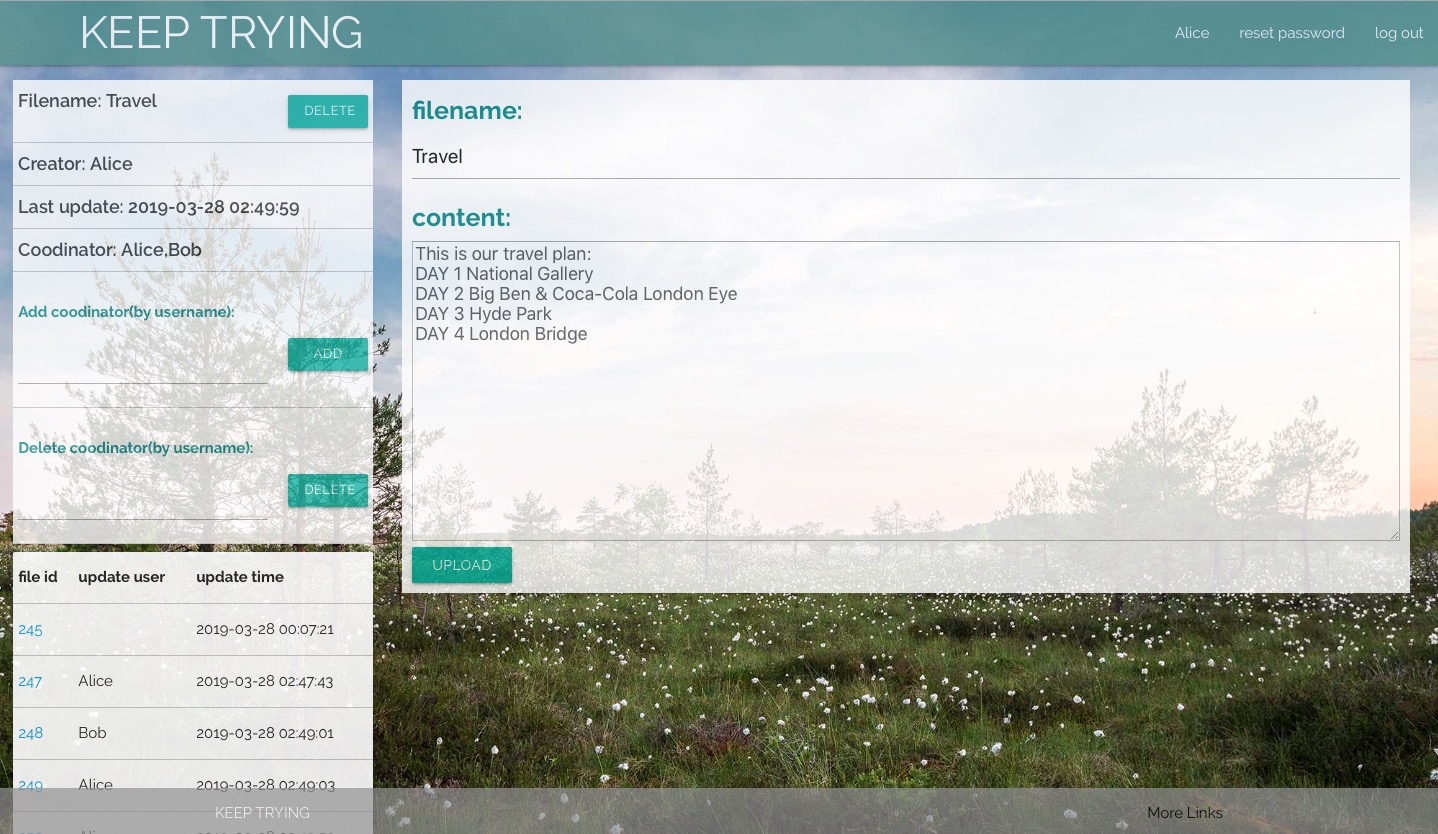
\includegraphics[width=.8\textwidth]{fileeditui.jpeg}
     \caption{File Edit Page}
     \label{edit}
     \end{figure}
    
    


\noindent Comparison Interface Introduction
\vspace{0.2cm}
\newline \noindent This is the comparison page when conflicts exist. 

  \begin{figure}[H]
     \centering
     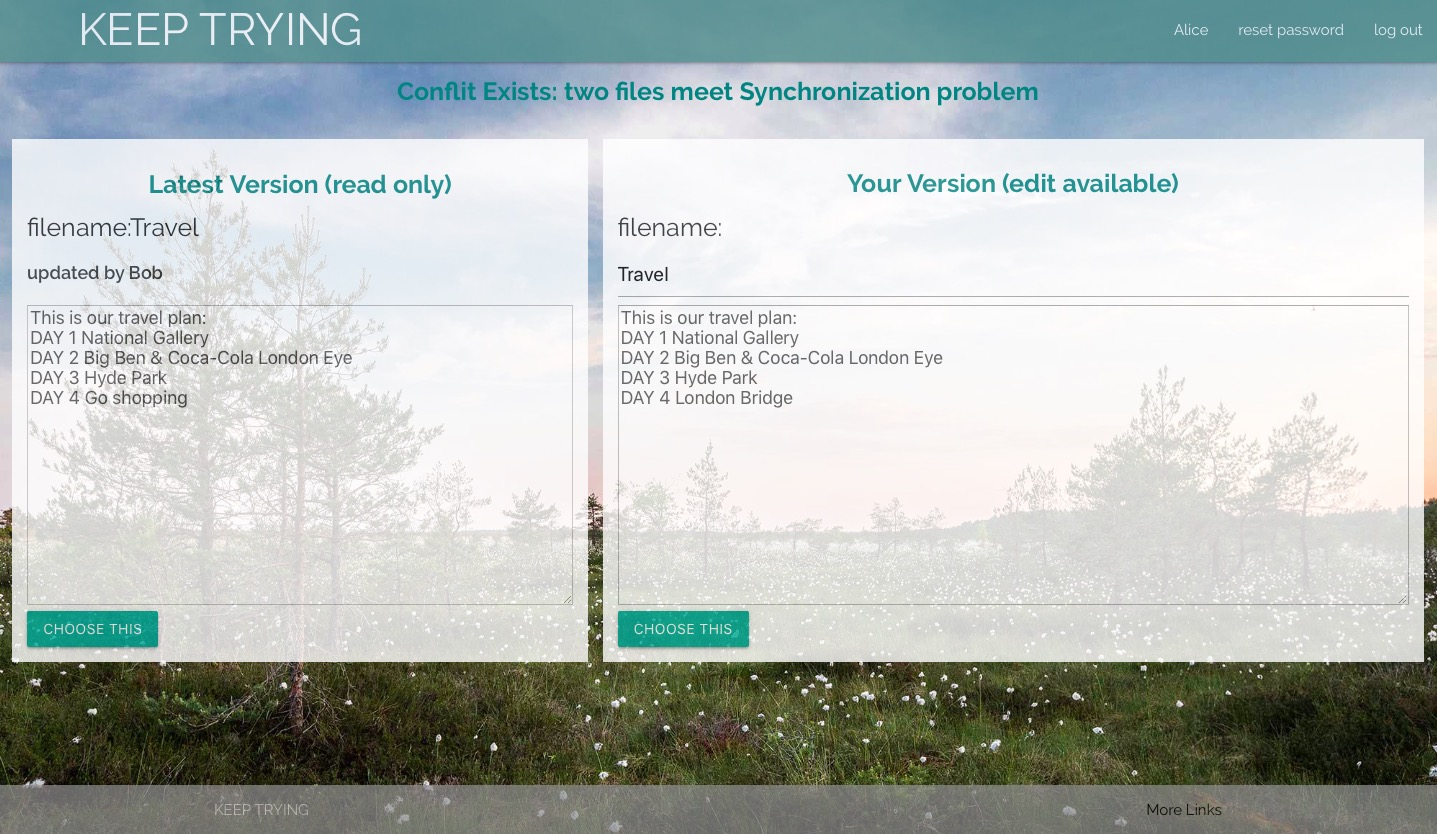
\includegraphics[width=.8\textwidth]{compare.jpeg}
     \caption{comparison page}
     \label{compare}
\end{figure}

  \begin{itemize}
      \item \textbf{Filename}: Simply shows the name of the file.
      \item \textbf{Your Version}: The version of the file when the current user is editing and the user can have editing authority.
      \item \textbf{Latest Version}: The user who login to this page only possess read permission, it shows the latest version of this file.
      \item \textbf{Choose Button}: Users can manually select the version they want to save and click this button to save.
  \end{itemize}
\noindent The final interface is shown is Fig.\ref{compare} 
%   \begin{figure}[H]
%      \centering
%      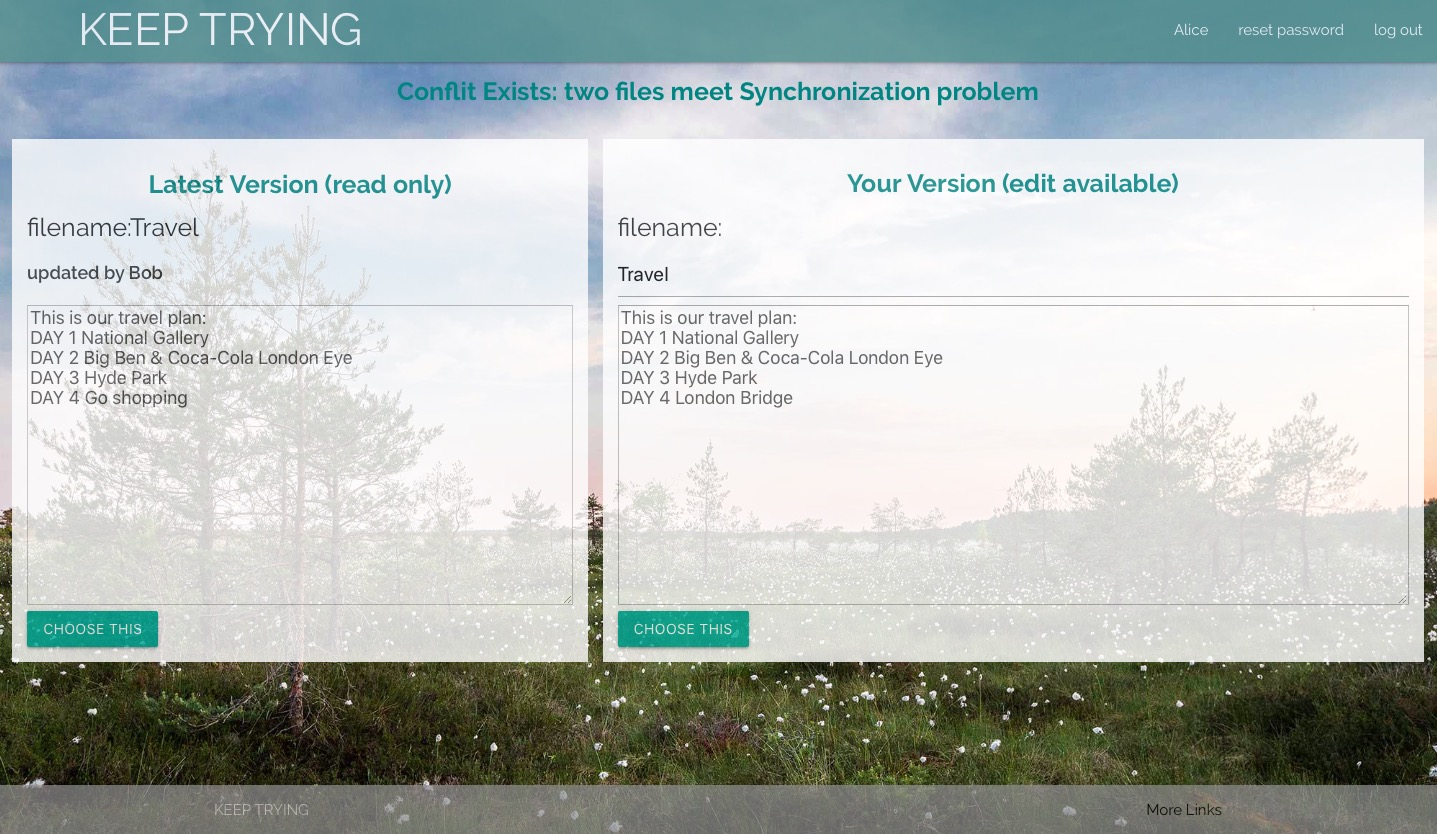
\includegraphics[width=.8\textwidth]{compare.jpeg}
%      \caption{comparison page}
%      \label{compare}
% \end{figure}
    

\subsubsection{iOS Mobile Client}
\noindent The main functions of iOS mobile client almost the same as the desktop client. And the final UI interface is shown in Fig.\ref{iuie} and the main page of 
access permissions is shown in Fig.\ref{au} .

  \begin{figure}[H]
     \centering
     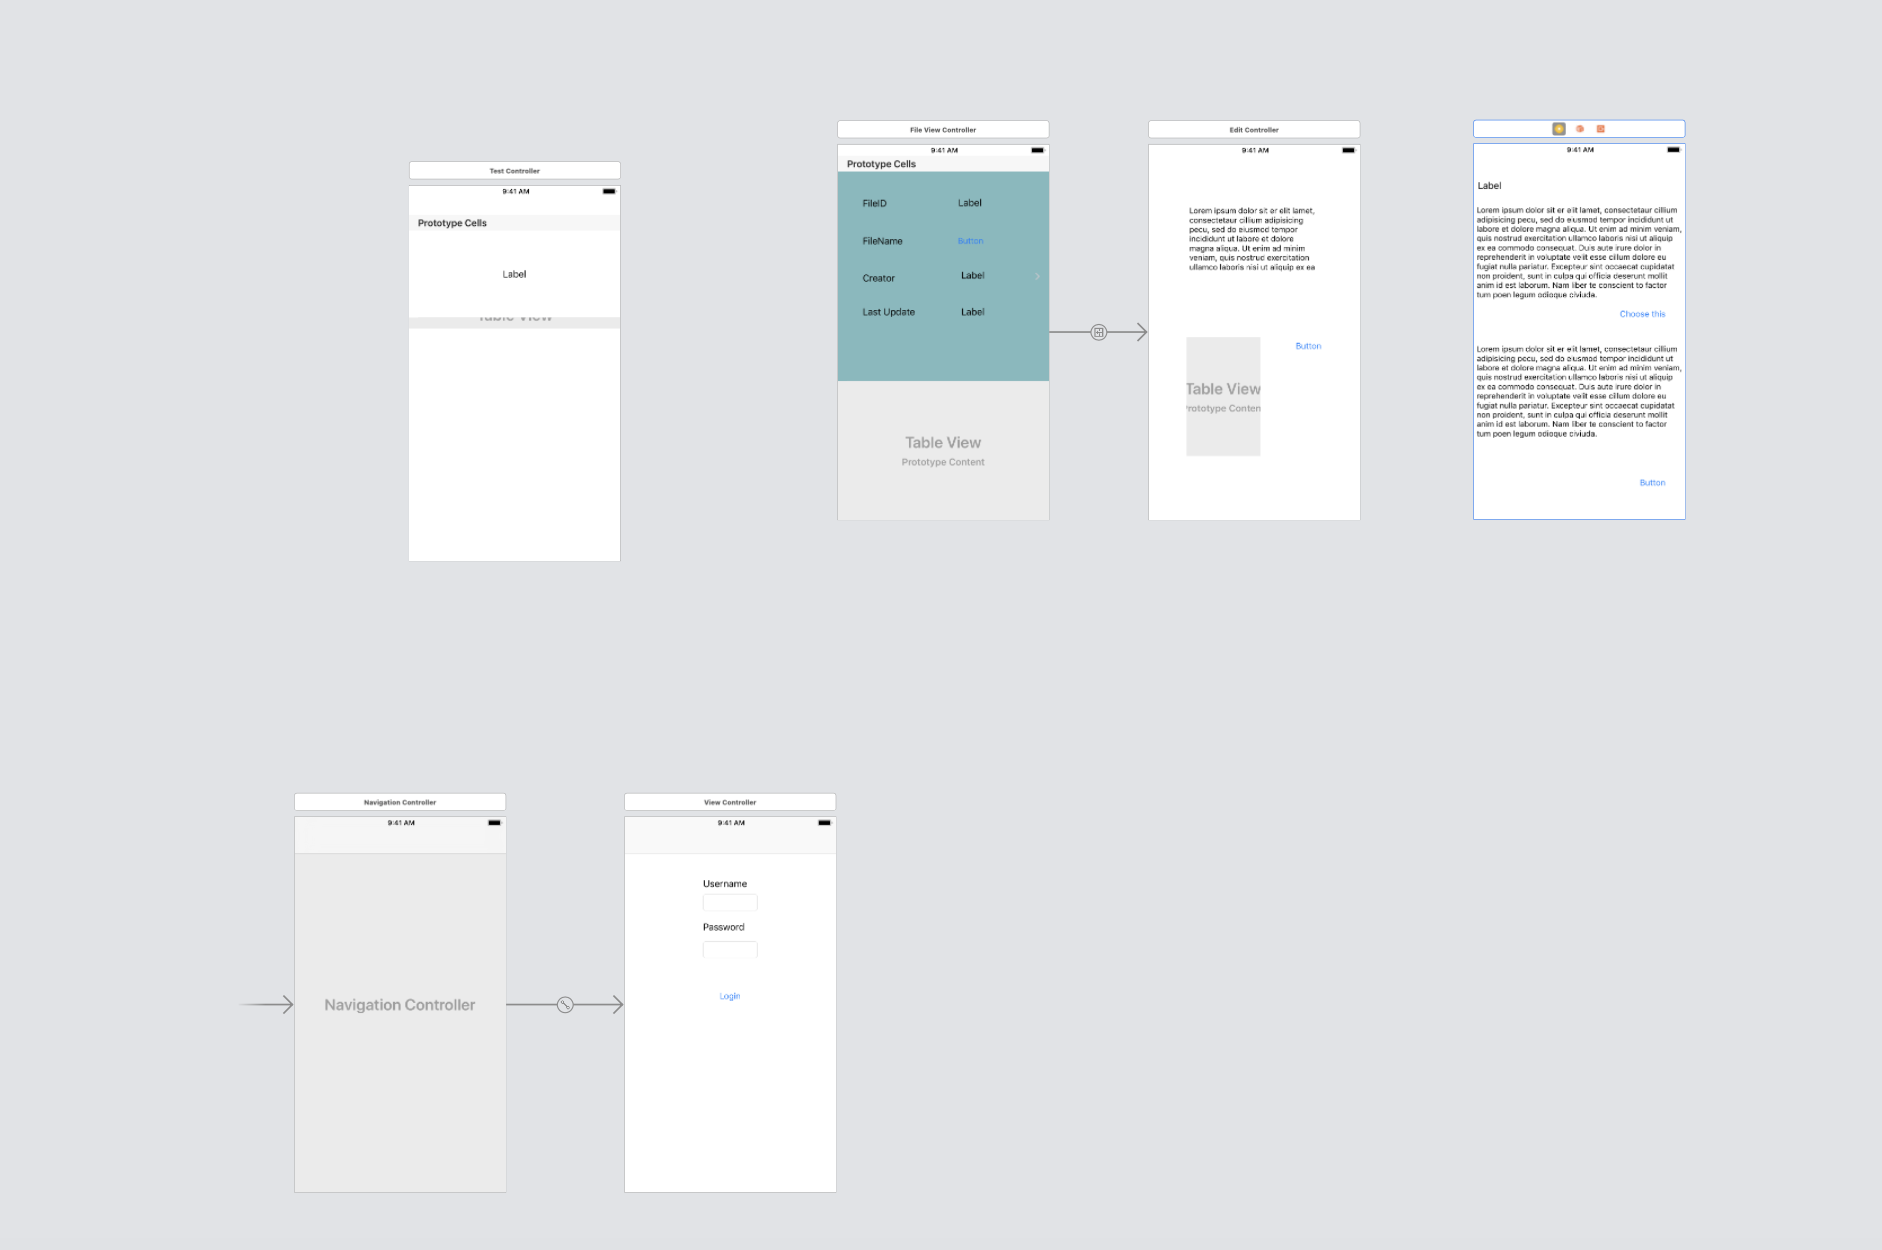
\includegraphics[width=.8\textwidth]{iui.png}
     \caption{iOS Client UI}
     \label{iuie}
\end{figure}

\begin{figure}[H]
  \centering
  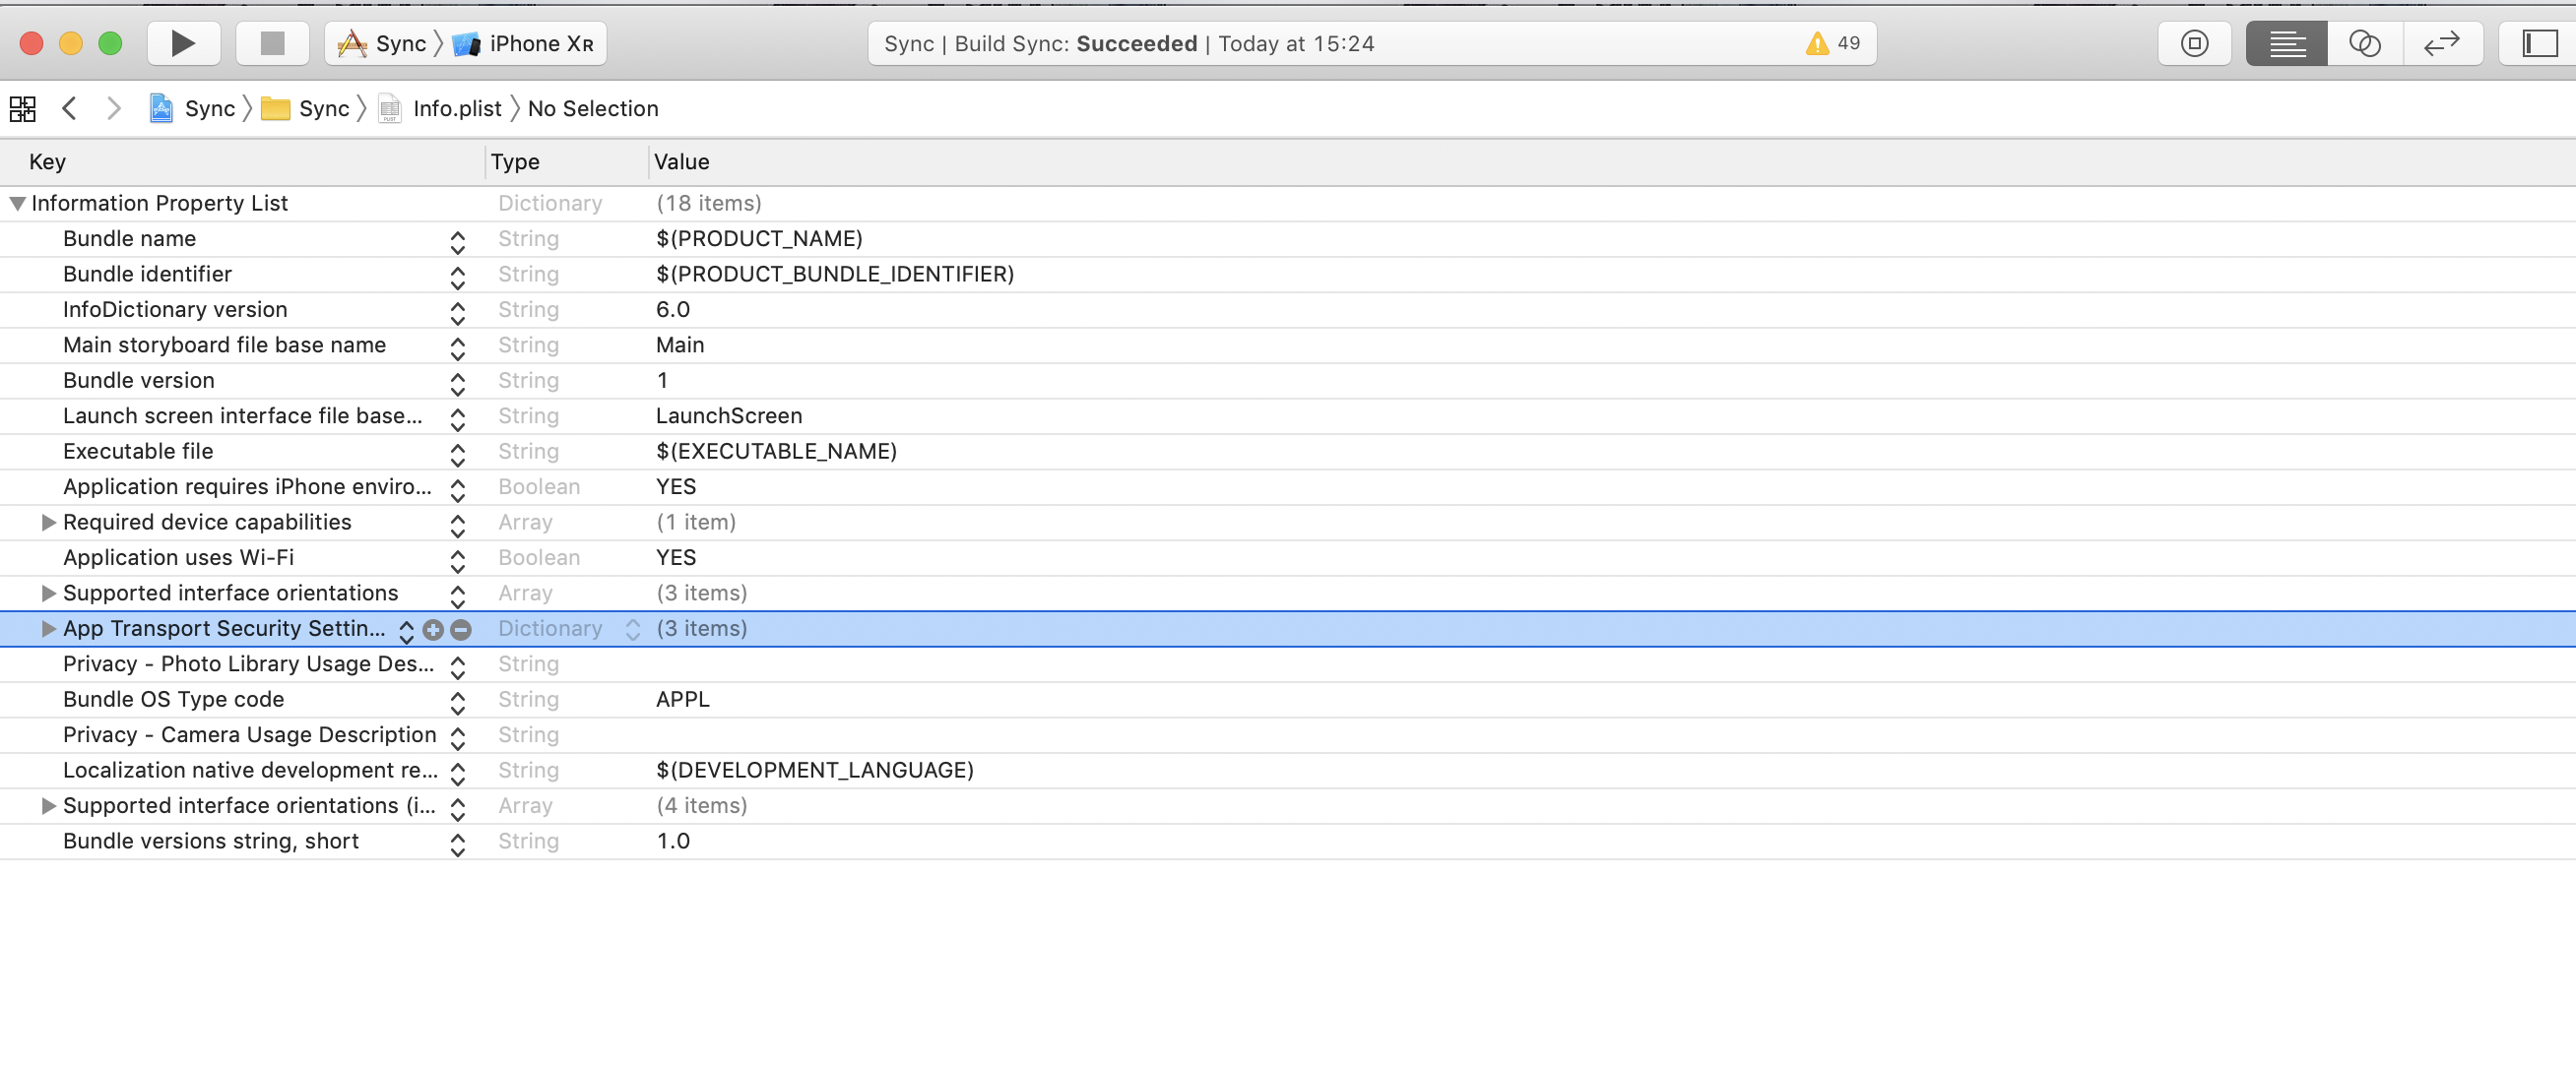
\includegraphics[width=.8\textwidth]{authset.png} %图片文件的相对路径
  \caption{List of iOS access permissions} %caption是图片的标题
  \label{au} %此处的label相当于一个图片的专属标志,目的是方便上下文的引用
\end{figure}





\subsection{Code Fragments and Explanation}
\subsubsection{Code Explanations of Desktop Client}
\noindent The code implementation of the registration function is shown in Fig.\ref{png1}. It first validates the user by requesting the \texttt{username} and the \texttt{password} from the user. The password must be 6-20 characters. After the validation, if the current user is not in the database, a new entry for the user will be created in the database user table with \texttt{create}. An ID is assigned to the user with \texttt{rand} function. After a successful registration, it will automatically jump to the login interface.

% The report must be at most 12,000 words or 35 pages (whichever is less)?超级爱你 我也爱你哦�� xin❤️xi��xin❤x❤️xi❤️❤️❤️nixnxin

\begin{figure}[H]
  \centering
  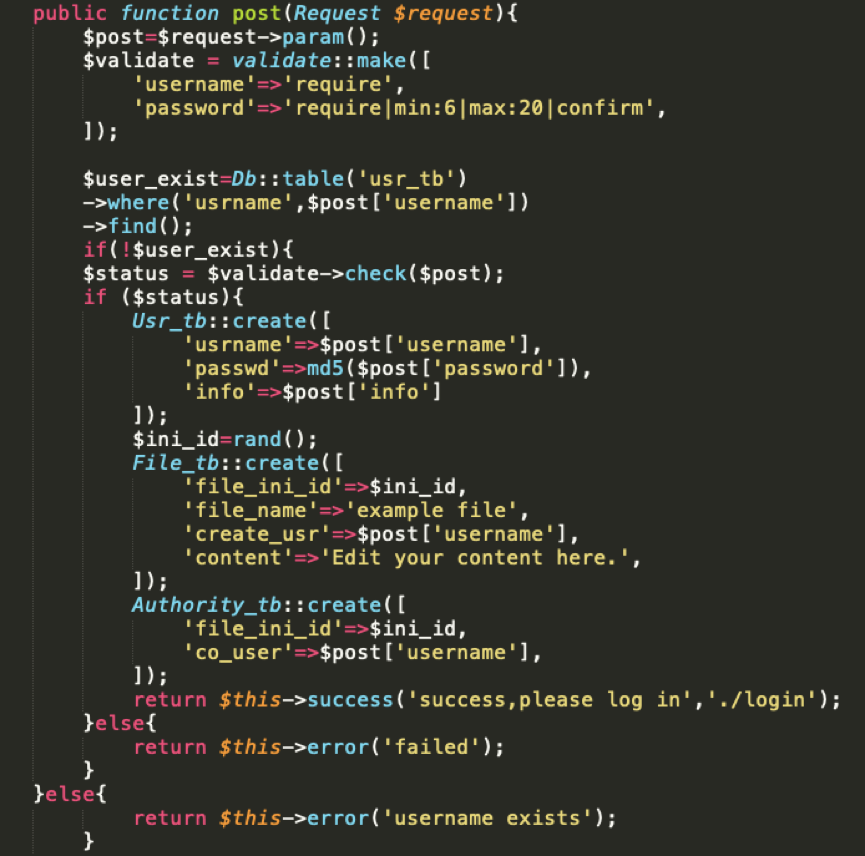
\includegraphics[width=.8\textwidth]{register.png} %图片文件的相对路径
  \caption{Code snippet of the registration function} %caption是图片的标题
  \label{png1} %此处的label相当于一个图片的专属标志,目的是方便上下文的引用
\end{figure}


\noindent The code implementation of the login function is shown in Fig.\ref{png2}. It first uses \texttt{IF} function to determine whether the user name received is the same as the username retrieved from the database. Then,the password is encrypted with \texttt{MD5} and the cipher text,which will be compared with the corresponding cipher in the session. Once the session values are equal, the user is verified to be successfully login and jumps automatically to the main web page(index.html).
\begin{figure}[H]
  \centering
  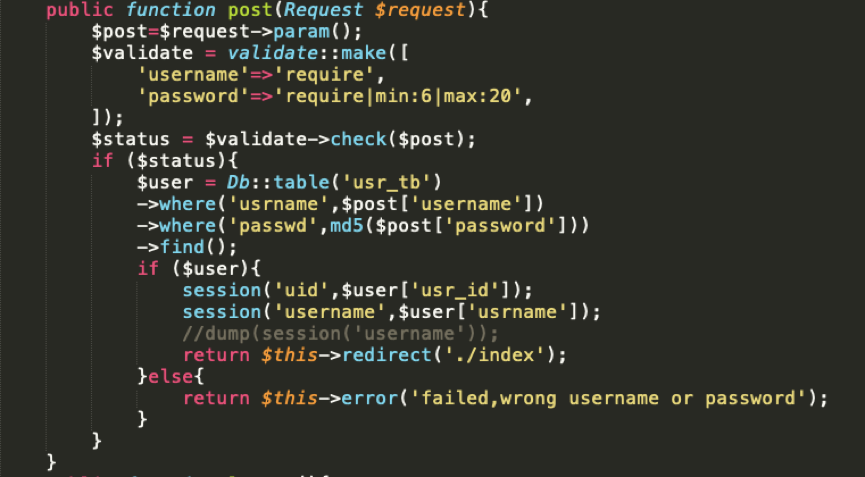
\includegraphics[width=.8\textwidth]{login.png} %图片文件的相对路径
  \caption{Code snippet of the login function} %caption是图片的标题
  \label{png2} %此处的label相当于一个图片的专属标志,目的是方便上下文的引用
\end{figure}

\noindent The code implementation of the file creation function is shown in Fig.\ref{png3}. It first generate and allocate file id by using \texttt{rand},then the database allocates space to this new file as well as update the permissions in the authority table.
\begin{figure}[H]
  \centering 
  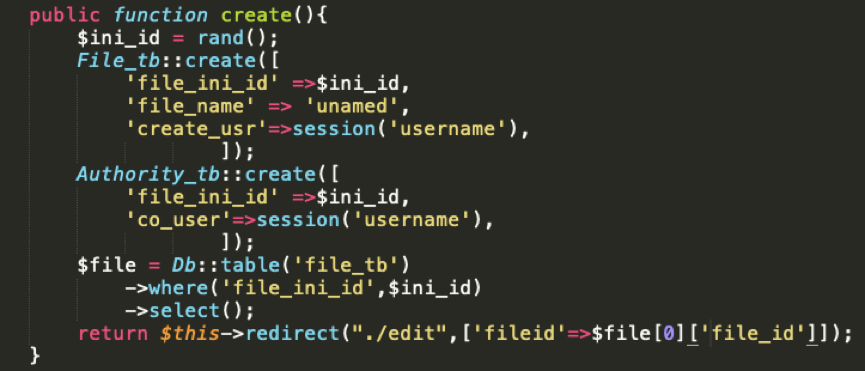
\includegraphics[width=.8\textwidth]{createfile.png} %图片文件的相对路径
  \caption{Code snippet of the file creation function} %caption是图片的标题
  \label{png3} %此处的label相当于一个图片的专属标志,目的是方便上下文的引用
\end{figure}



\noindent The code implementation of the file upload function is shown in Fig.\ref{png4}.The function of this code is to upload the existing local file to the database in the server.In detail,first and the most,it use the \texttt{IF}function to restrict the file type and size.After getting the local file path and extracting the contents of the file with \texttt{file\_get\_contents},it also randomly generates \texttt{file\_id}for the file.Finally, all the information relate to this file will be stored into the database.
\begin{figure}[H]
  \centering
  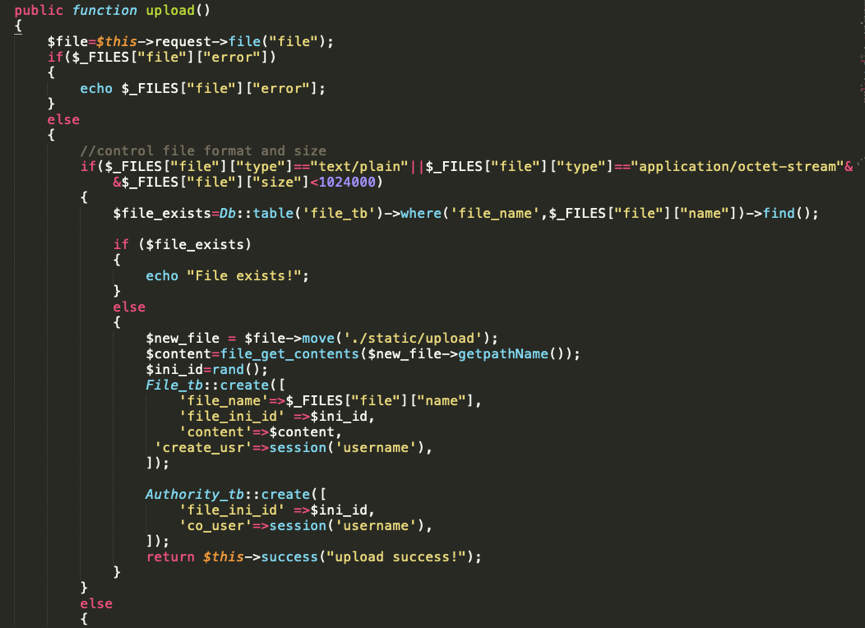
\includegraphics[width=.8\textwidth]{upnowfile.png} %图片文件的相对路径
  \caption{Code snippet of the file upload function} %caption是图片的标题
  \label{png4} %此处的label相当于一个图片的专属标志,目的是方便上下文的引用
\end{figure}


\noindent The code implementation of the file edit function is shown in Fig.\ref{png5}.In this edit interface, click \texttt{upload} to enter this function. Determine if there is a version error, if it does not exist, update the data to the database; if it exists, insert the data into the database and enter the compare page.

\begin{figure}[H]
  \centering
  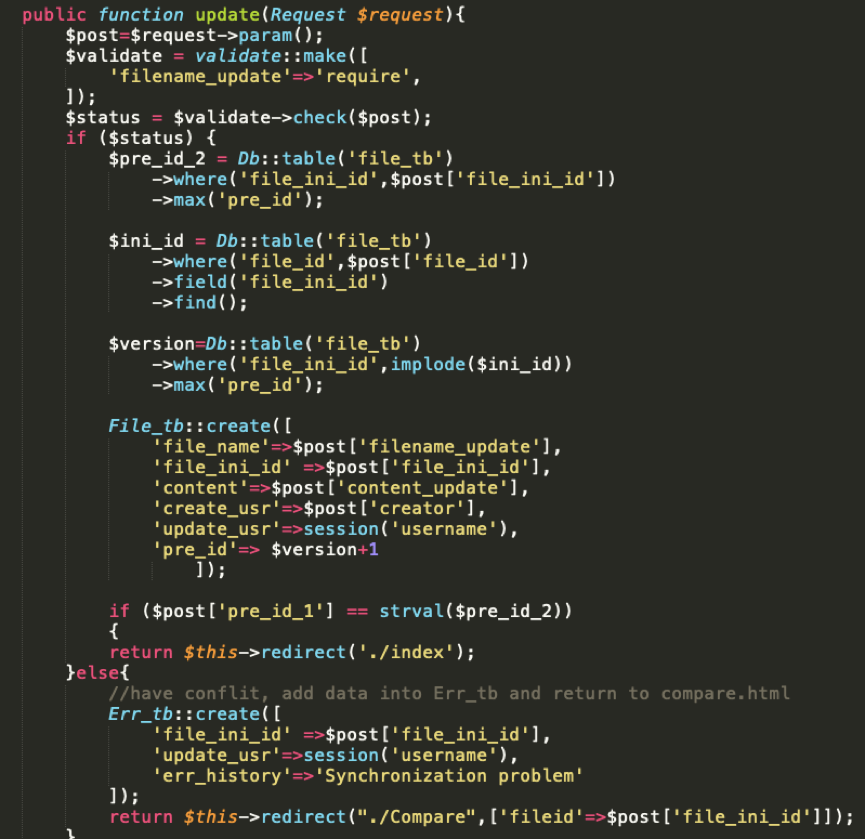
\includegraphics[width=.8\textwidth]{edit.png} %图片文件的相对路径
  \caption{Code snippet of the file edit function} %caption是图片的标题
  \label{png5} %此处的label相当于一个图片的专属标志,目的是方便上下文的引用
\end{figure}


\noindent The code implementation of adding coordinator function is shown in Fig.\ref{png6}.After determining whether there is a \texttt{username} to be added in \texttt{co\_user}, the system will operate differently depending on the particular case. If the coordinator already exists in database, it will not be added. If it does not exist, add this user into the permission table.
\begin{figure}[H]
  \centering
  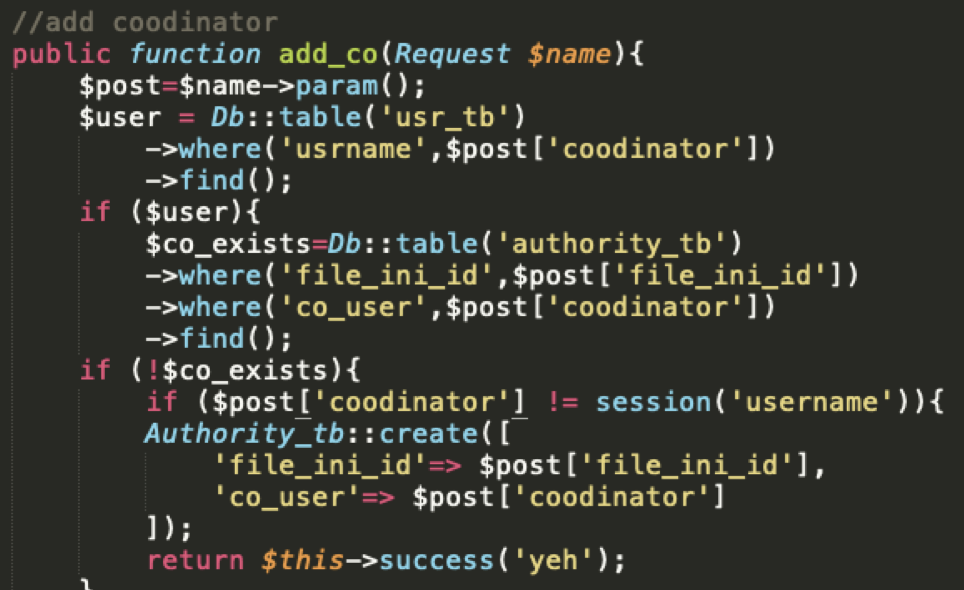
\includegraphics[width=.8\textwidth]{addco.png} %图片文件的相对路径
  \caption{Code snippet of adding coordinator function} %caption是图片的标题
  \label{png6} %此处的label相当于一个图片的专属标志,目的是方便上下文的引用
\end{figure}

\noindent The code implementation of Frontend modification permission function is shown in Fig.\ref{png7}.First, the if statement is used to determine that only the creator of the file will have the add and delete buttons. We can delete the edit authentication by their \texttt{username}.
\begin{figure}[H]
  \centering
  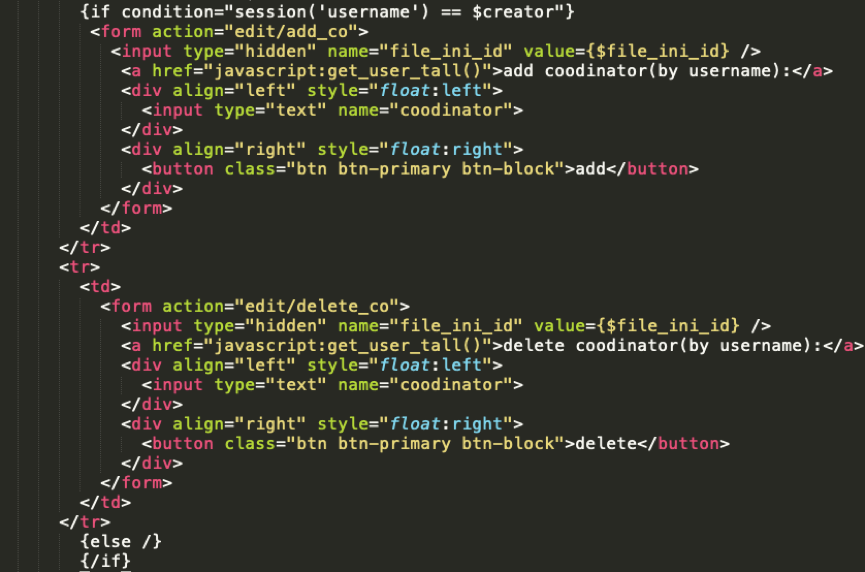
\includegraphics[width=.8\textwidth]{qianduan.png} %图片文件的相对路径
  \caption{} %caption是图片的标题
  \label{png7} %此处的label相当于一个图片的专属标志,目的是方便上下文的引用
\end{figure}



\noindent The code implementation of checking and returning to the historical version function is shown in Fig.\ref{png8}.
\begin{figure}[H]
  \centering
  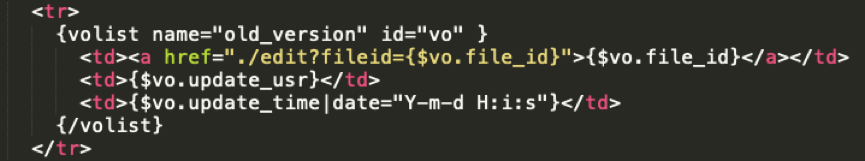
\includegraphics[width=.8\textwidth]{changeback.png} %图片文件的相对路径
  \caption{Code snippet of checking and returning to the historical version} %caption是图片的标题
  \label{png8} %此处的label相当于一个图片的专属标志,目的是方便上下文的引用
\end{figure}


\noindent The code implementation of checking and solving conflicts are shown separately in Fig.\ref{png9}.and Fig.\ref{png10}.This moment it have already encountered a conflict. According to the solution we designed, we need to construct a comparison page to compare the two conflicting documents together,and then, select the required version as the latest version according to the situation.
\noindent It gets the id of the file by using the \texttt{GET} command, then uses \texttt{fetch} to send the name and content of the two files to the compare page.
\noindent In the compare interface, the user can clearly see the contents of the two files and manually determine the version they want to keep, then they can choose to save this version of the file as the latest version.The code snippet in Fig.\ref{png10} is an example of saving the previous version of the file. After resetting the file\_id by \texttt{redirect}, it will automatically return to the index page.
\begin{figure}[H]
  \centering
  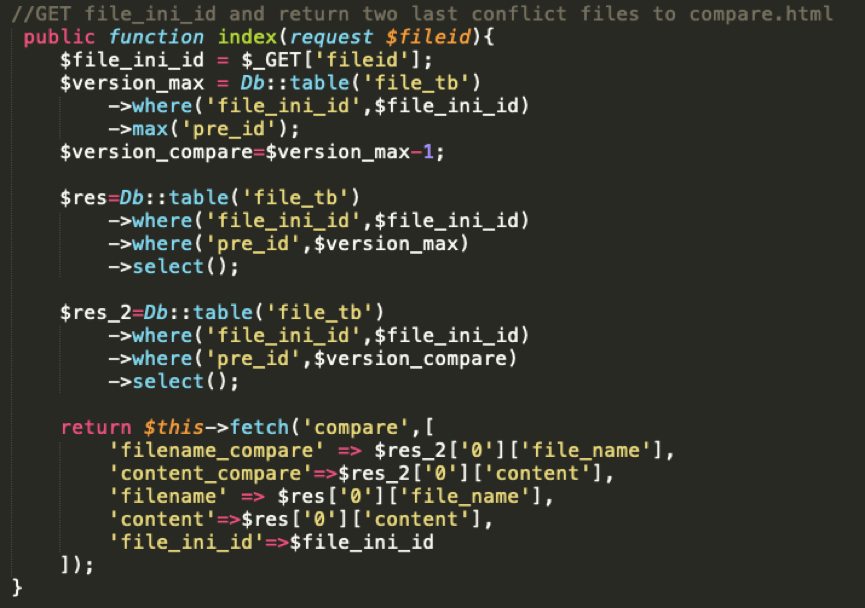
\includegraphics[width=.8\textwidth]{conflict.png}%图片文件的相对路径
  \caption{Code snippet of checking conflicts} %caption是图片的标题
  \label{png9} %此处的label相当于一个图片的专属标志,目的是方便上下文的引用
\end{figure}

\begin{figure}[H]
  \centering
  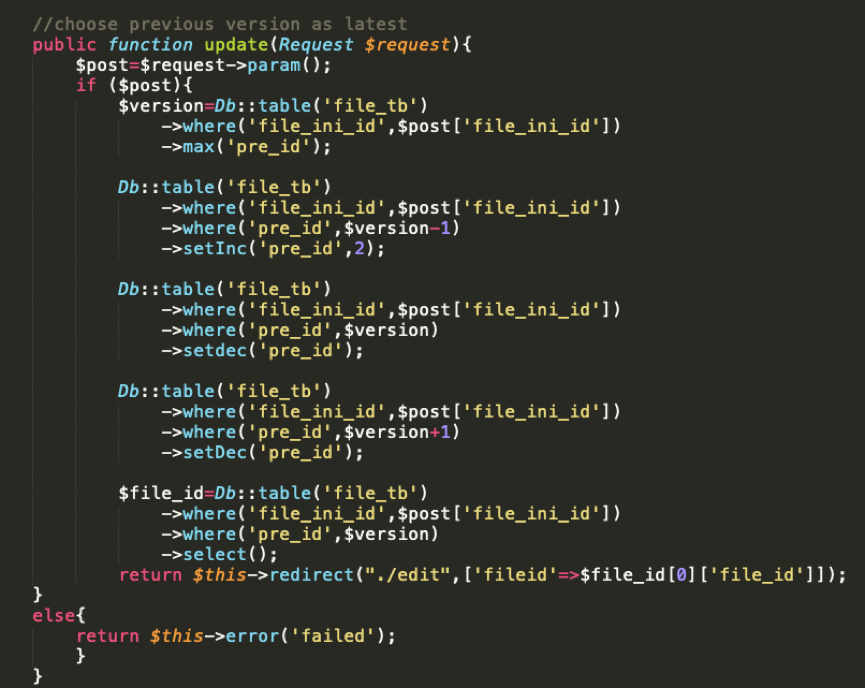
\includegraphics[width=.8\textwidth]{conflictsolve.png}%图片文件的相对路径
  \caption{Code snippet of saving the previous version} %caption是图片的标题
  \label{png10} %此处的label相当于一个图片的专属标志,目的是方便上下文的引用
\end{figure}




\subsubsection{Code Explanations of iOS Mobile Client}
\noindent The code implementation of request from HTTP and analyze JSON is shown in Fig.\ref{png12}. It first use alamonfire to request from HTTP which include URL, method, parameters, encoding, headers and interceptor. When the system gets JSON database, it uses ObjectMapper to analyze the data and change it into a data array. It will also send to the view controller when the app receives a memory warning.

\begin{figure}[H]
  \centering
  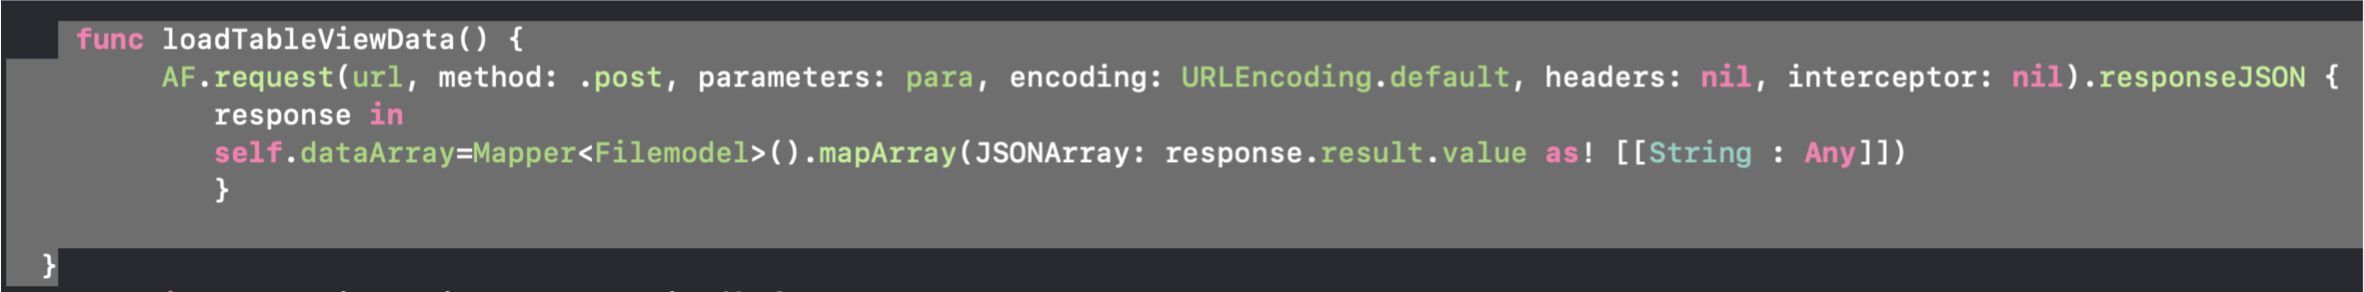
\includegraphics[width=.8\textwidth]{ios.png} %图片文件的相对路径
  \caption{Code snippet of request from HTTP and analyze JASON} %caption是图片的标题
  \label{png12} %此处的label相当于一个图片的专属标志,目的是方便上下文的引用
\end{figure}




\vspace{0.3cm}
\noindent This page \ref{pss} contains specific code about how to set the users authorities.
\begin{figure}[H]
  \centering
  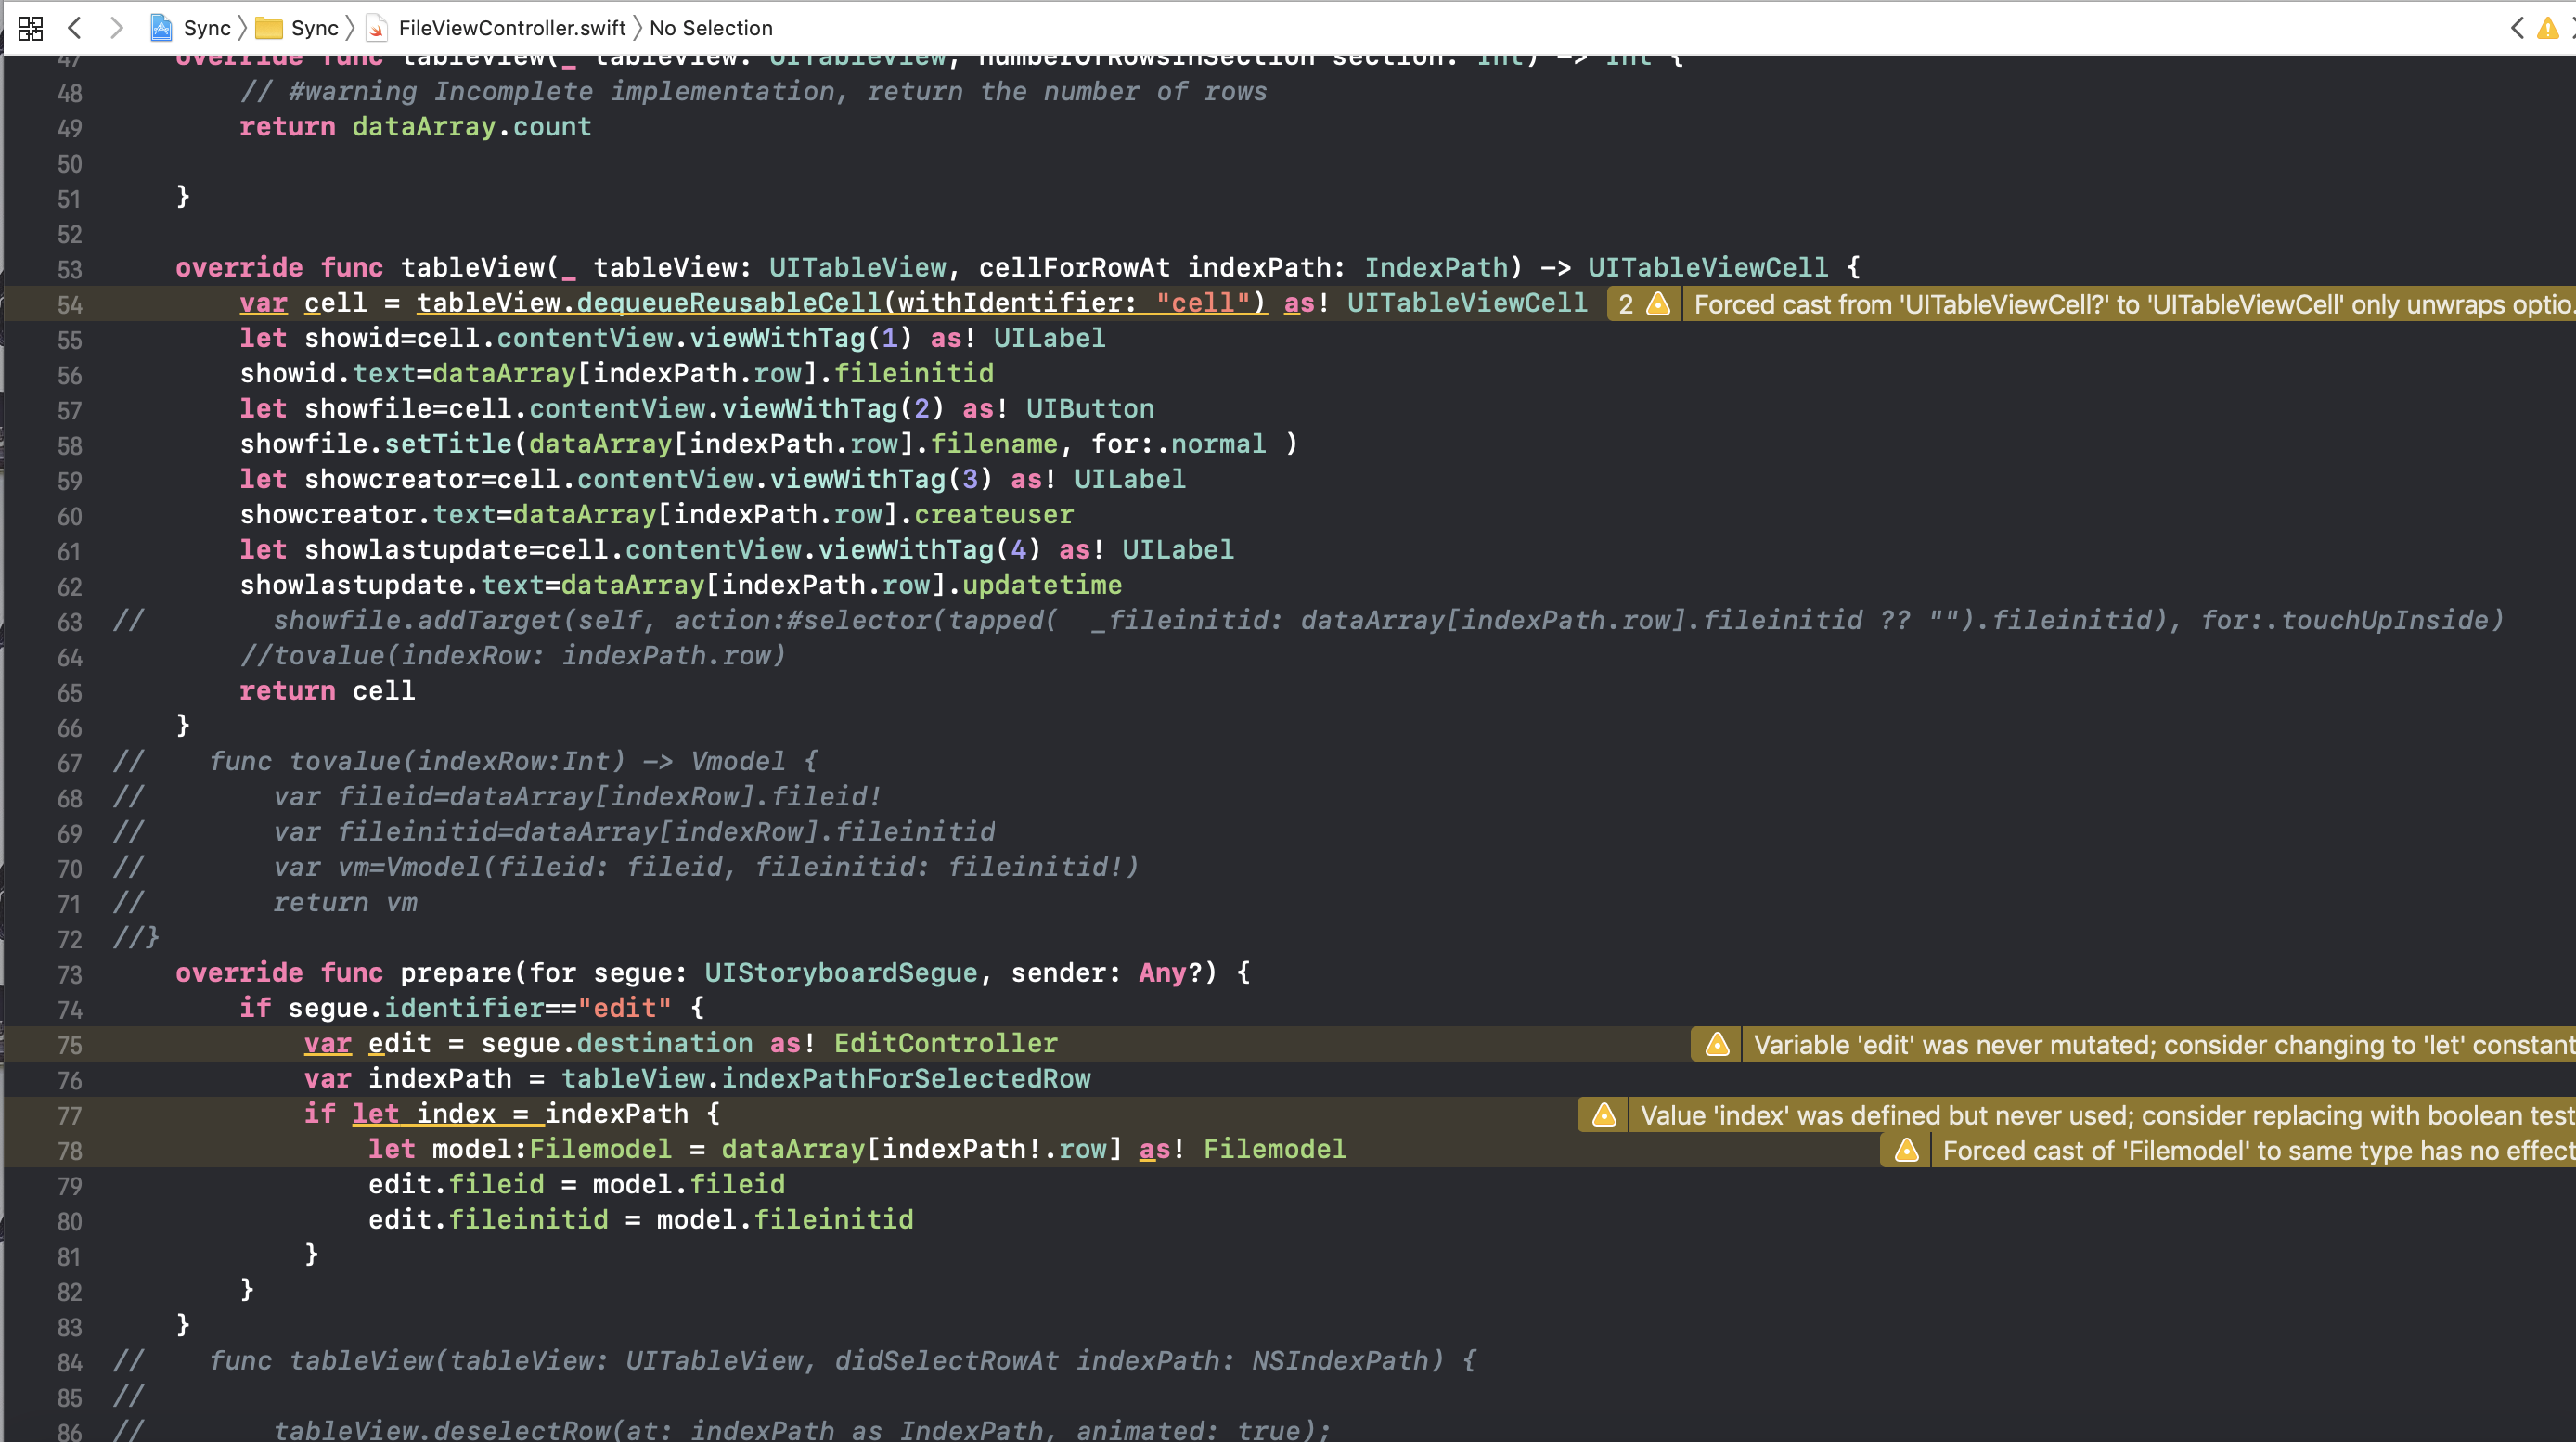
\includegraphics[width=.8\textwidth]{fv.png} %图片文件的相对路径
  \caption{Code snippet of set user authority} %caption是图片的标题
  \label{pss} %此处的label相当于一个图片的专属标志,目的是方便上下文的引用
\end{figure}

\vspace{0.3cm}
\noindent The code implementation of the Converting JSONArray and Model arrays using Object library is shown in Fig.\ref{ccc} and Fig.\ref{cc1}. These code use \texxxt{UITableView} to display a list of files and pass parameters between the view controller via \texxxt{segue}.
\begin{figure}[H]
  \centering
  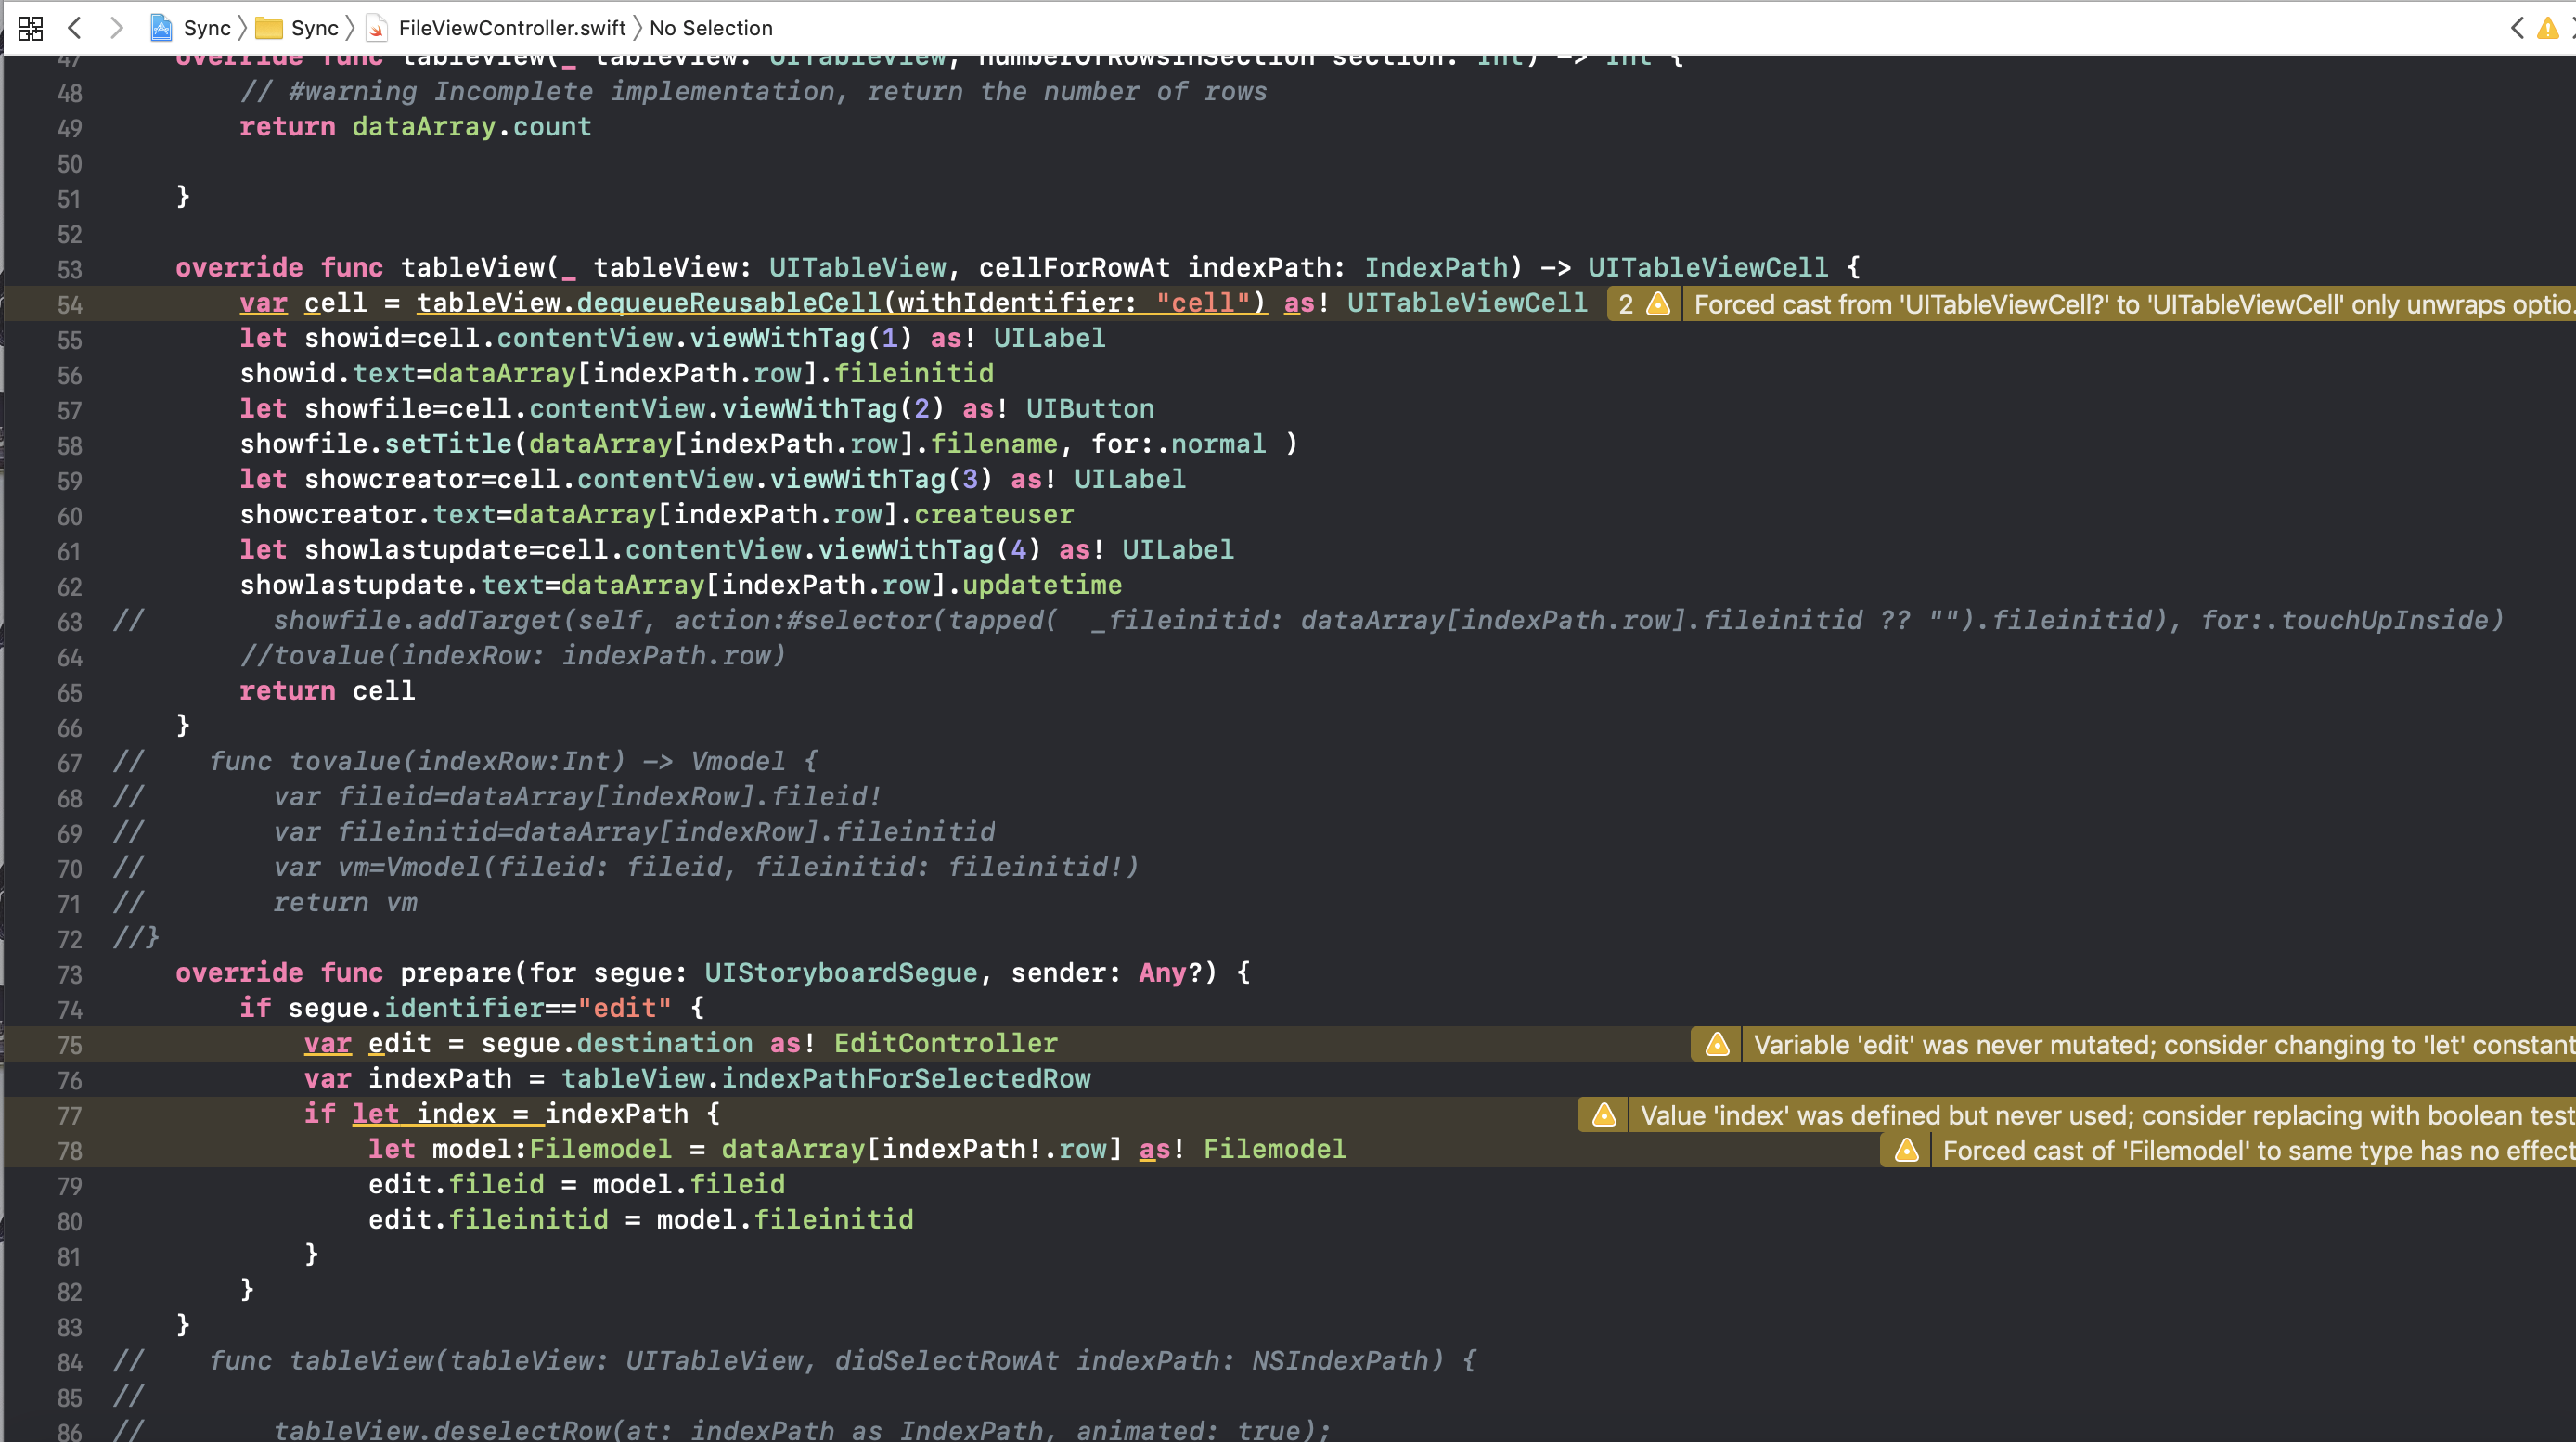
\includegraphics[width=.8\textwidth]{c1.png}%图片文件的相对路径
  \caption{Code snippet of Converting JSONArray and Model arrays} %caption是图片的标题
  \label{ccc} %此处的label相当于一个图片的专属标志,目的是方便上下文的引用
\end{figure}

\begin{figure}[H]
  \centering
  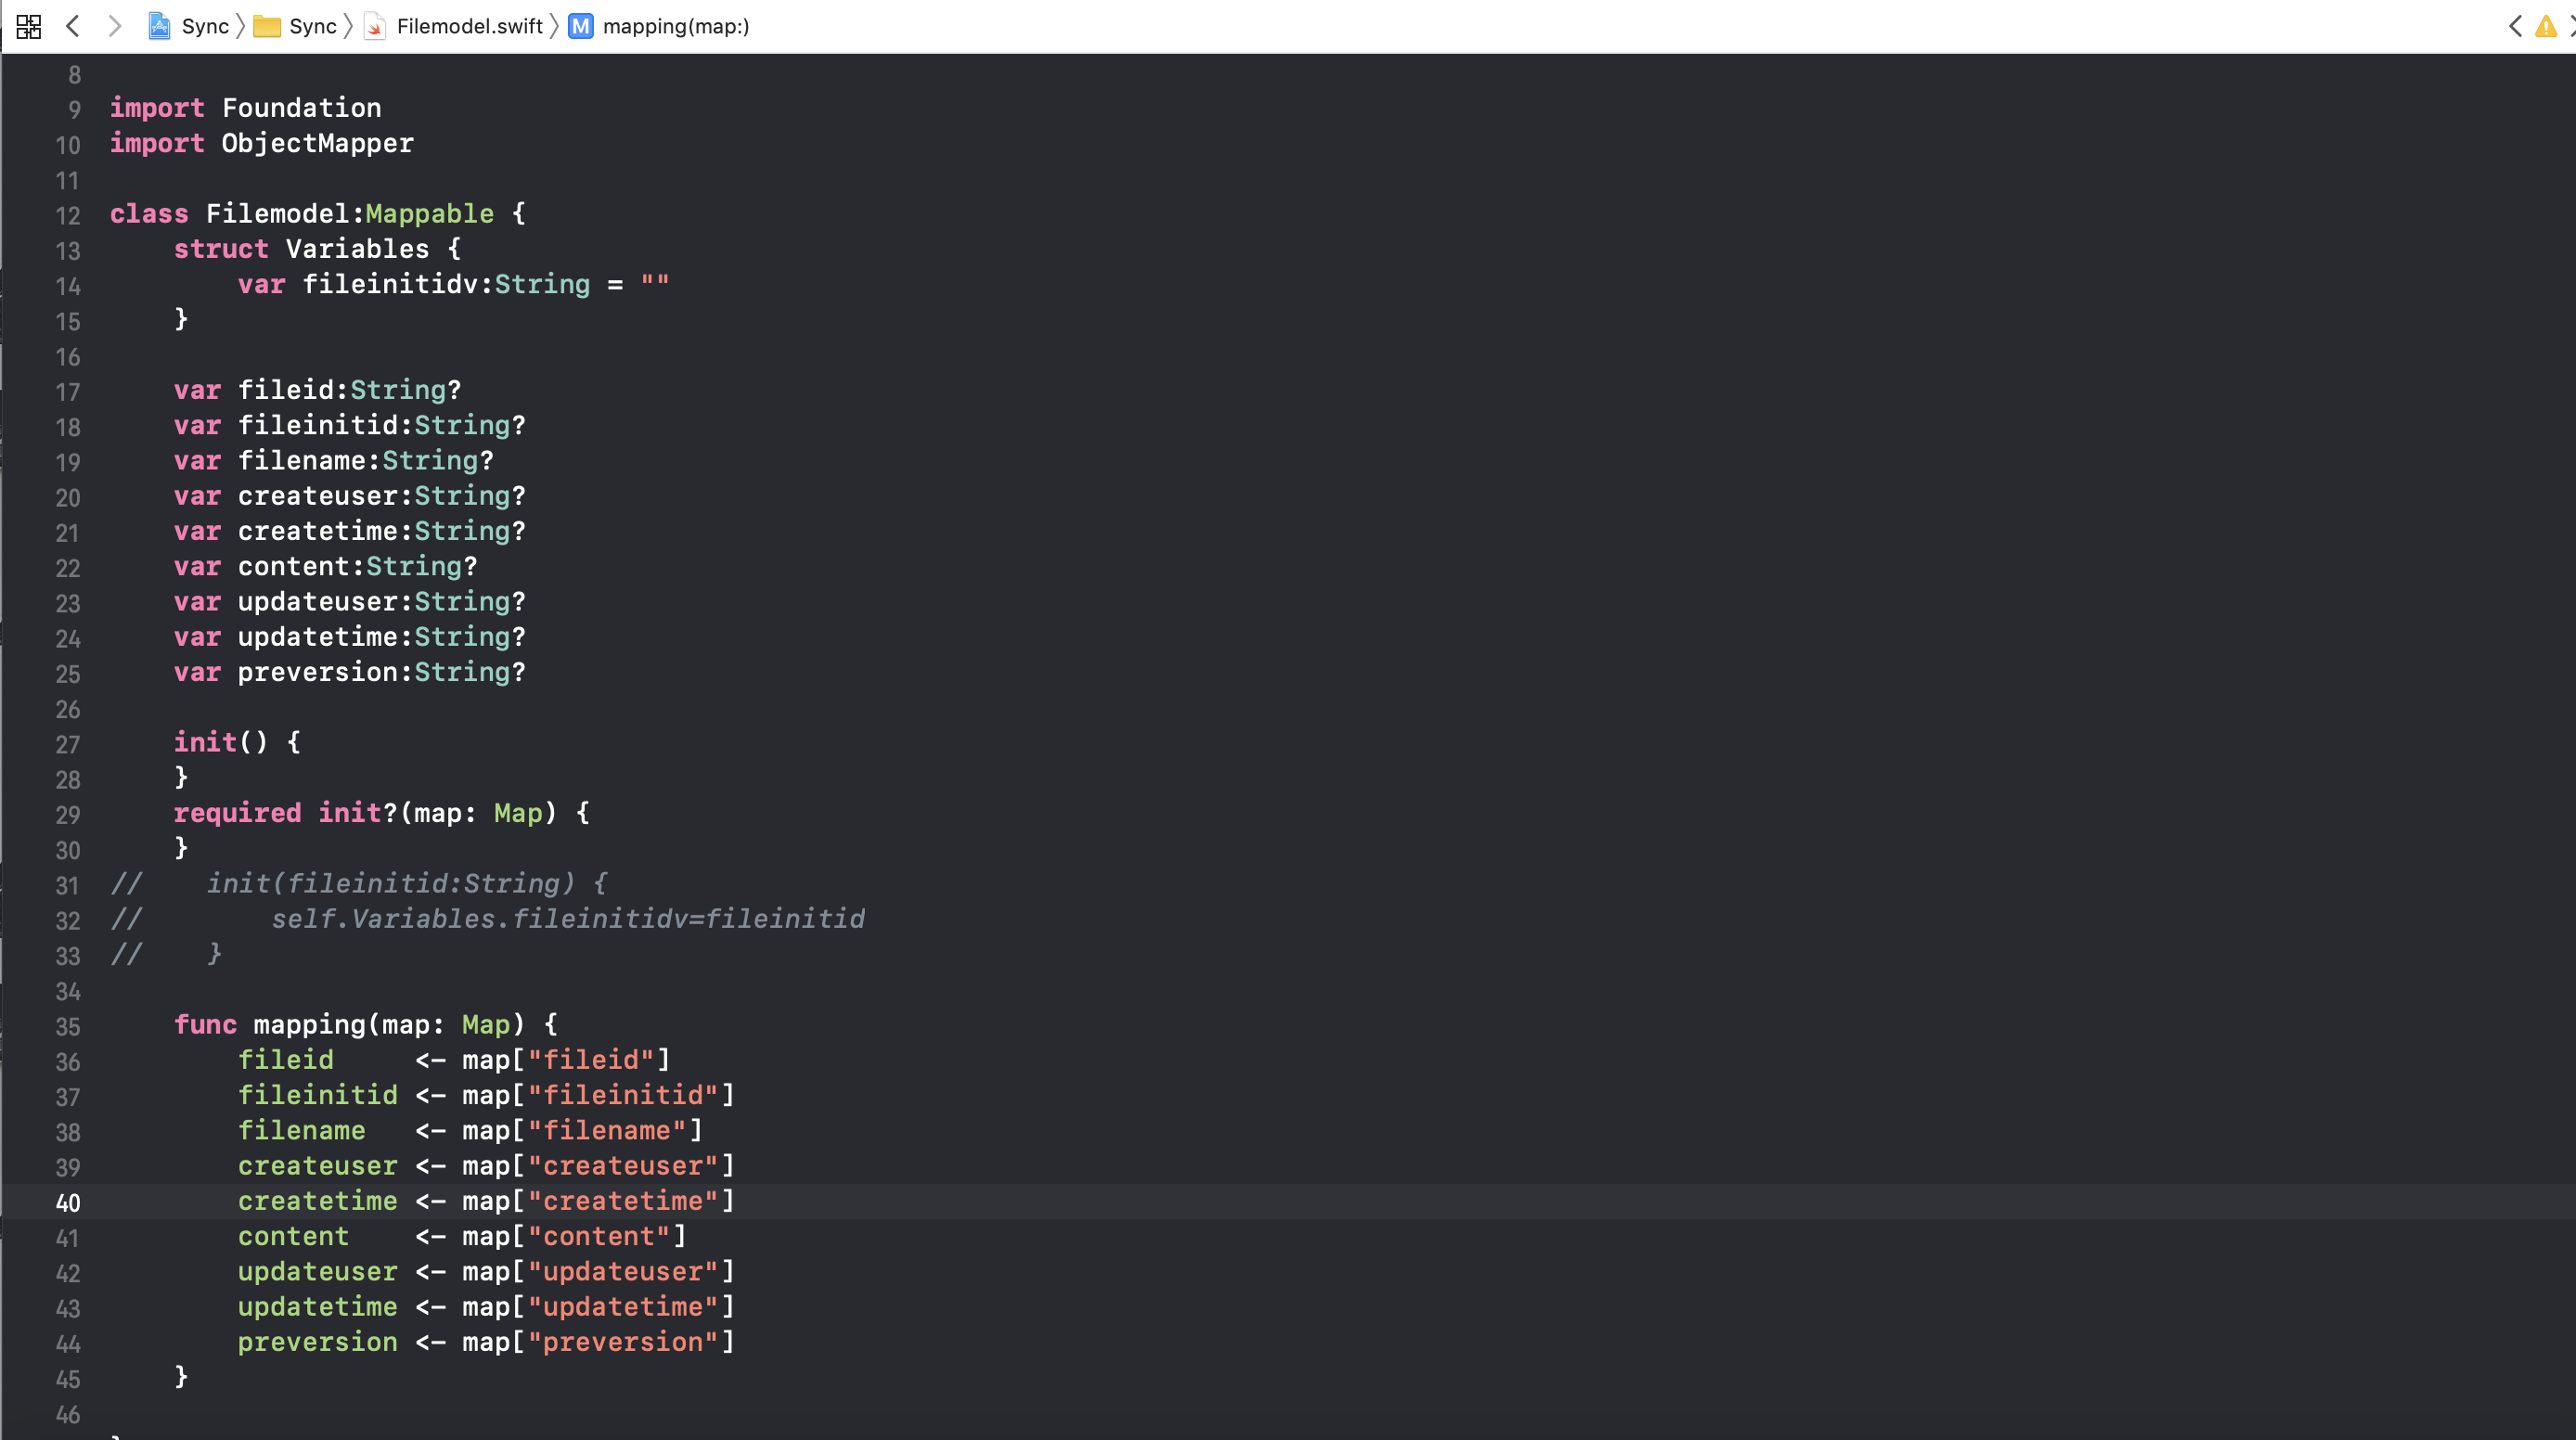
\includegraphics[width=.8\textwidth]{c2.png}%图片文件的相对路径
  \caption{Code snippet of Converting JSONArray and Model arrays} %caption是图片的标题
  \label{cc1} %此处的label相当于一个图片的专属标志,目的是方便上下文的引用
\end{figure}

\noindent The code implementation of returning data in the background is shown in Fig.\ref{aaa}. These code Use Just framework, which is an open source framework based on the Http NetWorking component, written in swift language to process http requests to exchange data with the background server, the background returns json-based bytes.
\begin{figure}[H]
  \centering
  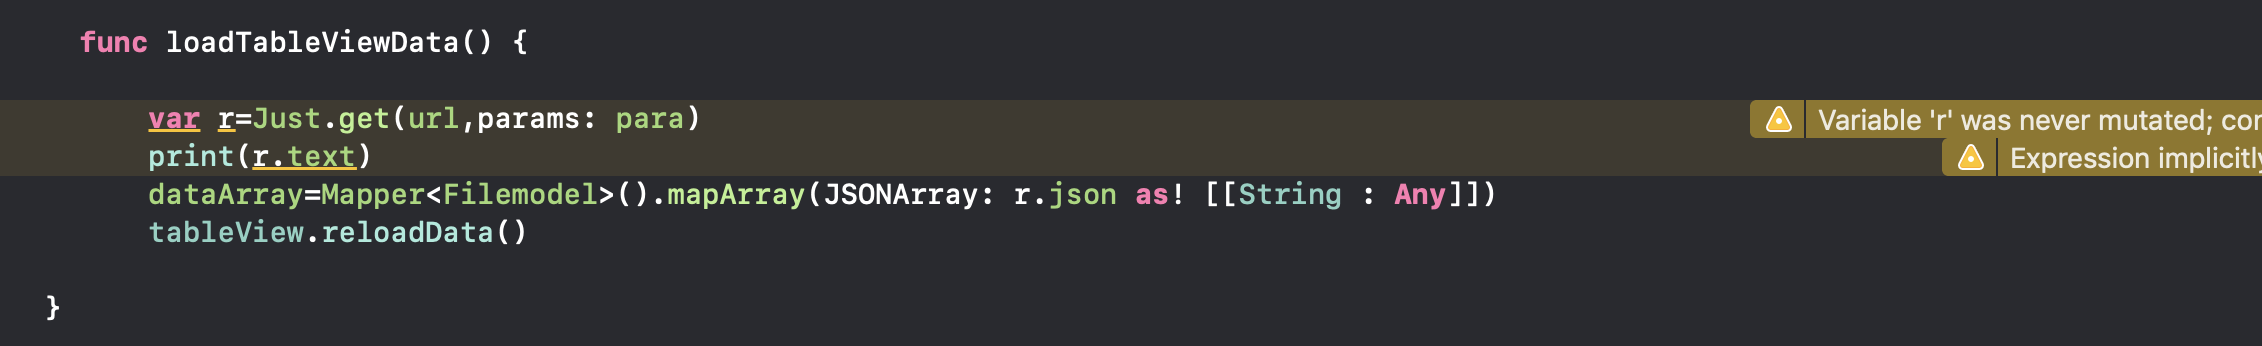
\includegraphics[width=.8\textwidth]{just.png}%图片文件的相对路径
  \caption{Code snippet of returning data in the background} %caption是图片的标题
  \label{aaa} %此处的label相当于一个图片的专属标志,目的是方便上下文的引用
\end{figure}

\vspace{0.3cm}
\noindent The code implementation of connecting database is shown in Fig.\ref{aa}.

\begin{figure}[H]
  \centering
  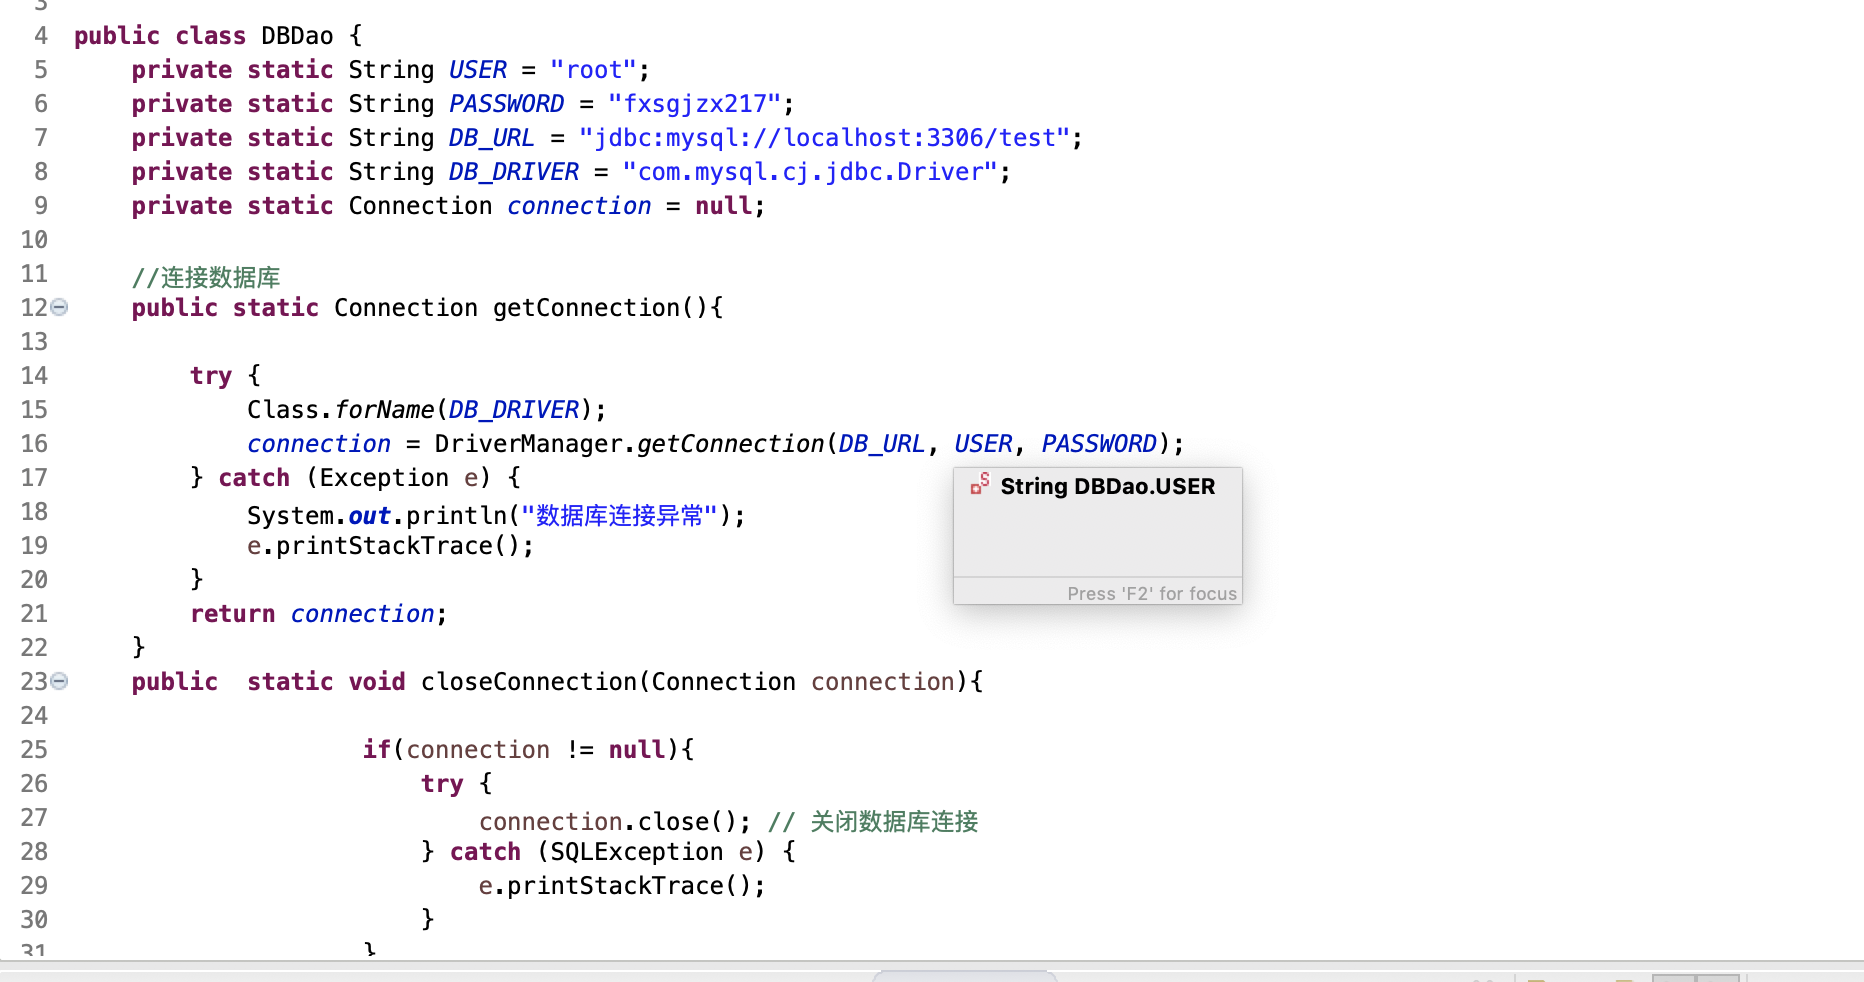
\includegraphics[width=.8\textwidth]{lianjie.png}%图片文件的相对路径
  \caption{Code snippet of Database linkage} %caption是图片的标题
  \label{aa} %此处的label相当于一个图片的专属标志,目的是方便上下文的引用
\end{figure}

\vspace{0.3cm}
\noindent The code implementation of how to get users information is shown in Fig.\ref{a1a}. It shows how to complete the settings and the acquisition of user information.

\begin{figure}[H]
  \centering
  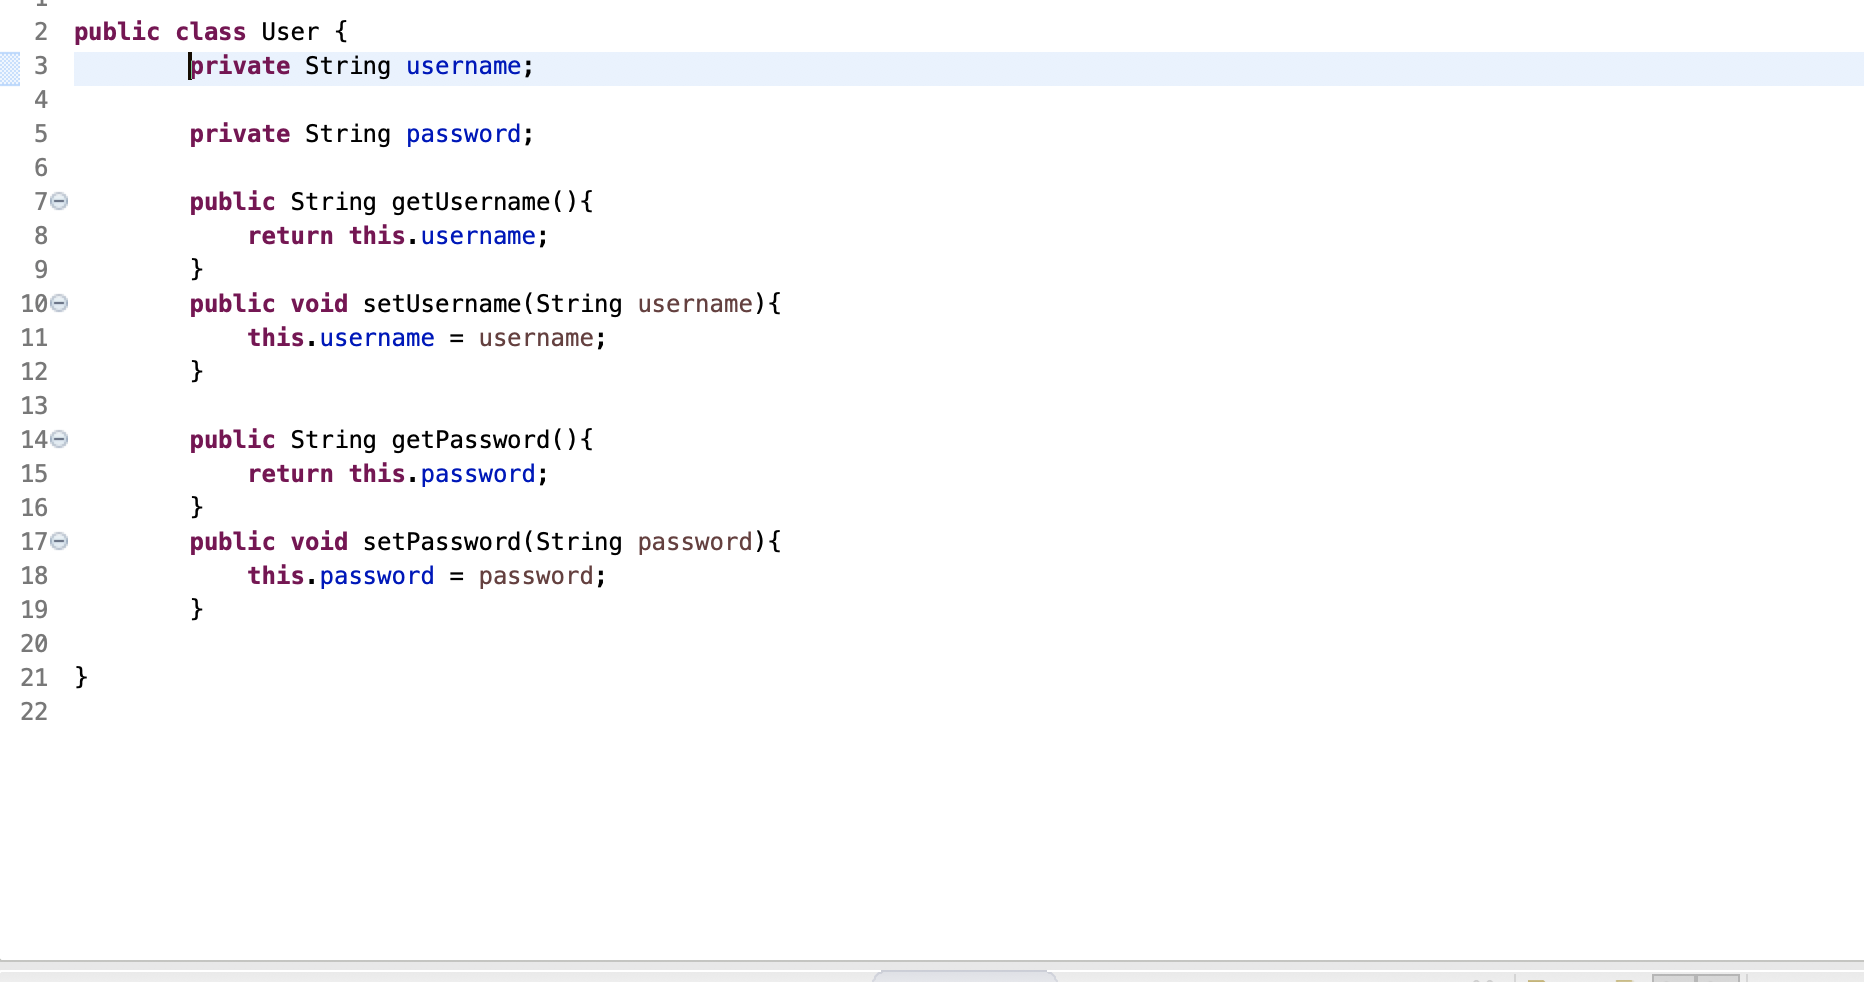
\includegraphics[width=.8\textwidth]{USERMODEL.png}%图片文件的相对路径
  \caption{Code snippet of the User Model} %caption是图片的标题
  \label{a1a} %此处的label相当于一个图片的专属标志,目的是方便上下文的引用
\end{figure}

\vspace{0.3cm}
\noindent The code implementation of how to compare file versions with \texttt{TestView} is shown in Fig.\ref{brian}. 

\begin{figure}[H]
  \centering
  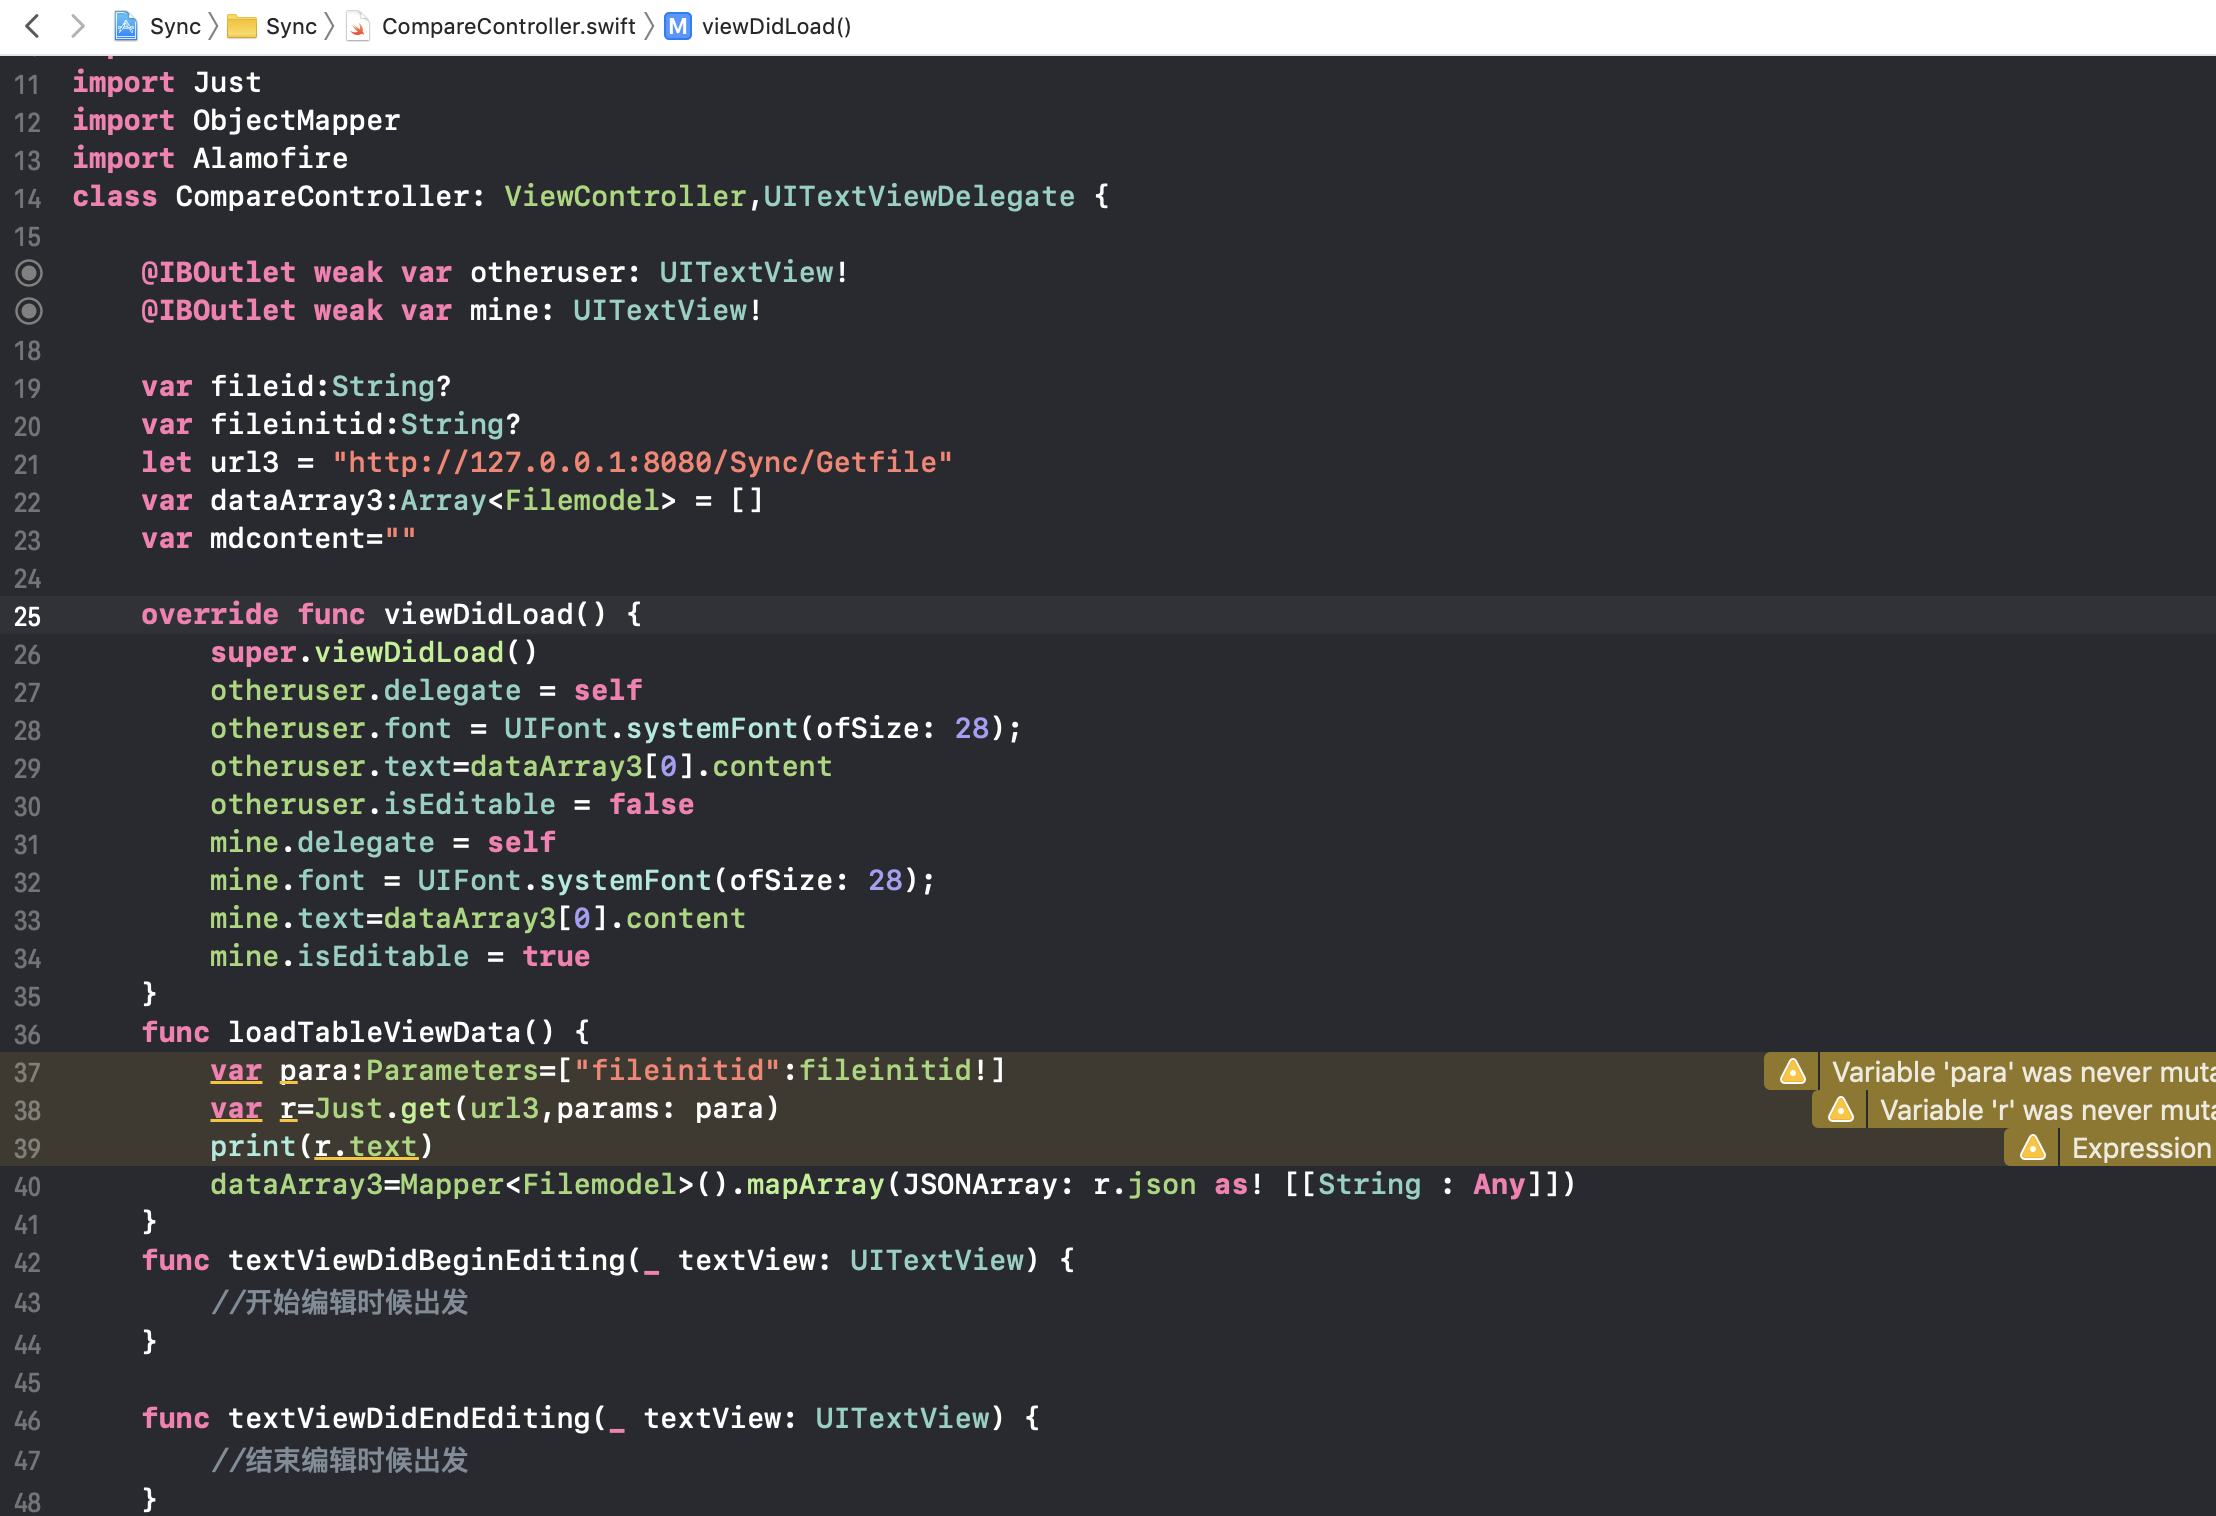
\includegraphics[width=.8\textwidth]{view.png}%图片文件的相对路径
  \caption{Code snippet of User Model} %caption是图片的标题
  \label{brian} %此处的label相当于一个图片的专属标志,目的是方便上下文的引用
\end{figure}

\vspace{0.3cm}
\noindent The code implementation of how to use SQL statements in this software is shown below. Fig.\ref{brian2} shows how to insert users information and file contents, and Fig.\ref{brian3} explains how to use SQL statements to query files according to their version number.

\begin{figure}[H]
  \centering
  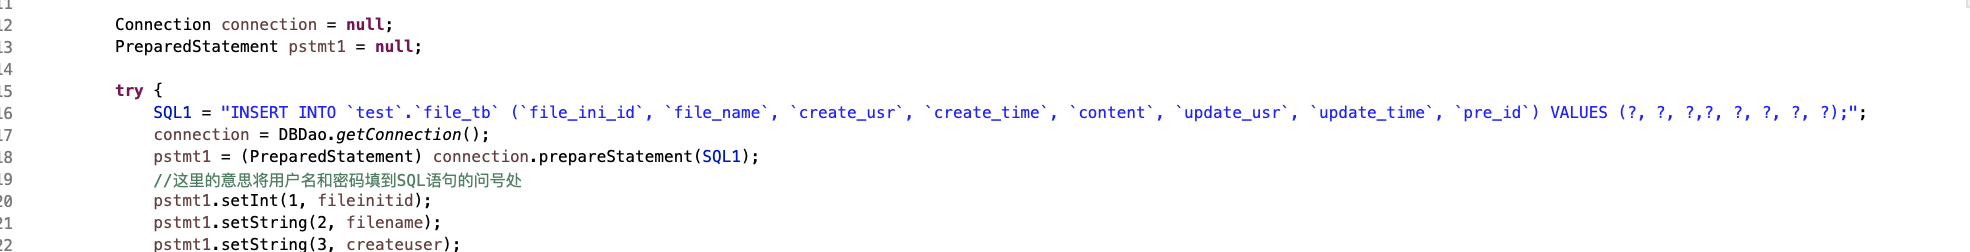
\includegraphics[width=.8\textwidth]{sql1.png}%图片文件的相对路径
  \caption{Code snippet of SQL statement 1} %caption是图片的标题
  \label{brian2} %此处的label相当于一个图片的专属标志,目的是方便上下文的引用
\end{figure}



\begin{figure}[H]
  \centering
  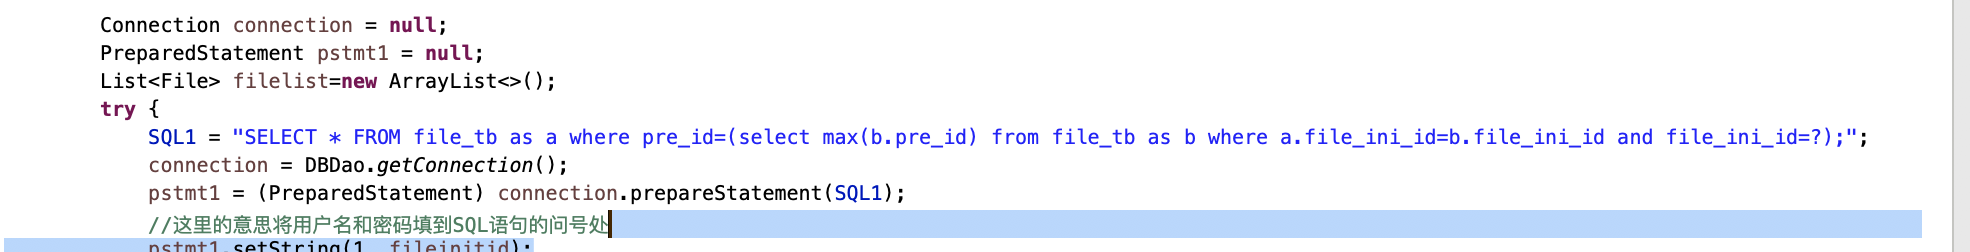
\includegraphics[width=.8\textwidth]{sql2.png}%图片文件的相对路径
  \caption{Code snippet of SQL statement 2} %caption是图片的标题
  \label{brian3} %此处的label相当于一个图片的专属标志,目的是方便上下文的引用
\end{figure}

\subsection{Software Testing}
\noindent In order to ensure that the system is working properly, we need to conduct a series of rigorous and effective tests to discover potential problems with the software. Web testing and iOS client testing vary from one carrier to another, so system testing and details are different. Web testing is B/S architecture and browser-based, in the contrary, iOS client testing is C/S architecture. We tested the both ends of our system, and more specific information will be  described as follows:

\vspace{0.3cm}
\noindent \textbf{Desktop Client Testing:}
\vspace{0.3cm}
\newline \noindent Our desktop client uses the ThinkPHP framework, but ThinkPHP itself does not provide the corresponding unit testing support, but we combined some of the functions in ThinkPHP into a library by learning from others' experience and ideas. This library can be used for unit testing of ThinkPHP to further ensure the quality of the software. The characteristics of this method are: easy to use, convenient and non-invasive.

\begin{itemize}
    \item Create a new folder test under the \texttt{Appcation}, and create a new test class named \texttt{IndexTest.php}.
    \item Concrete code implementation and annotation are showned in Fig.\ref{php}.
  
   \begin{figure}[H]
  \centering
  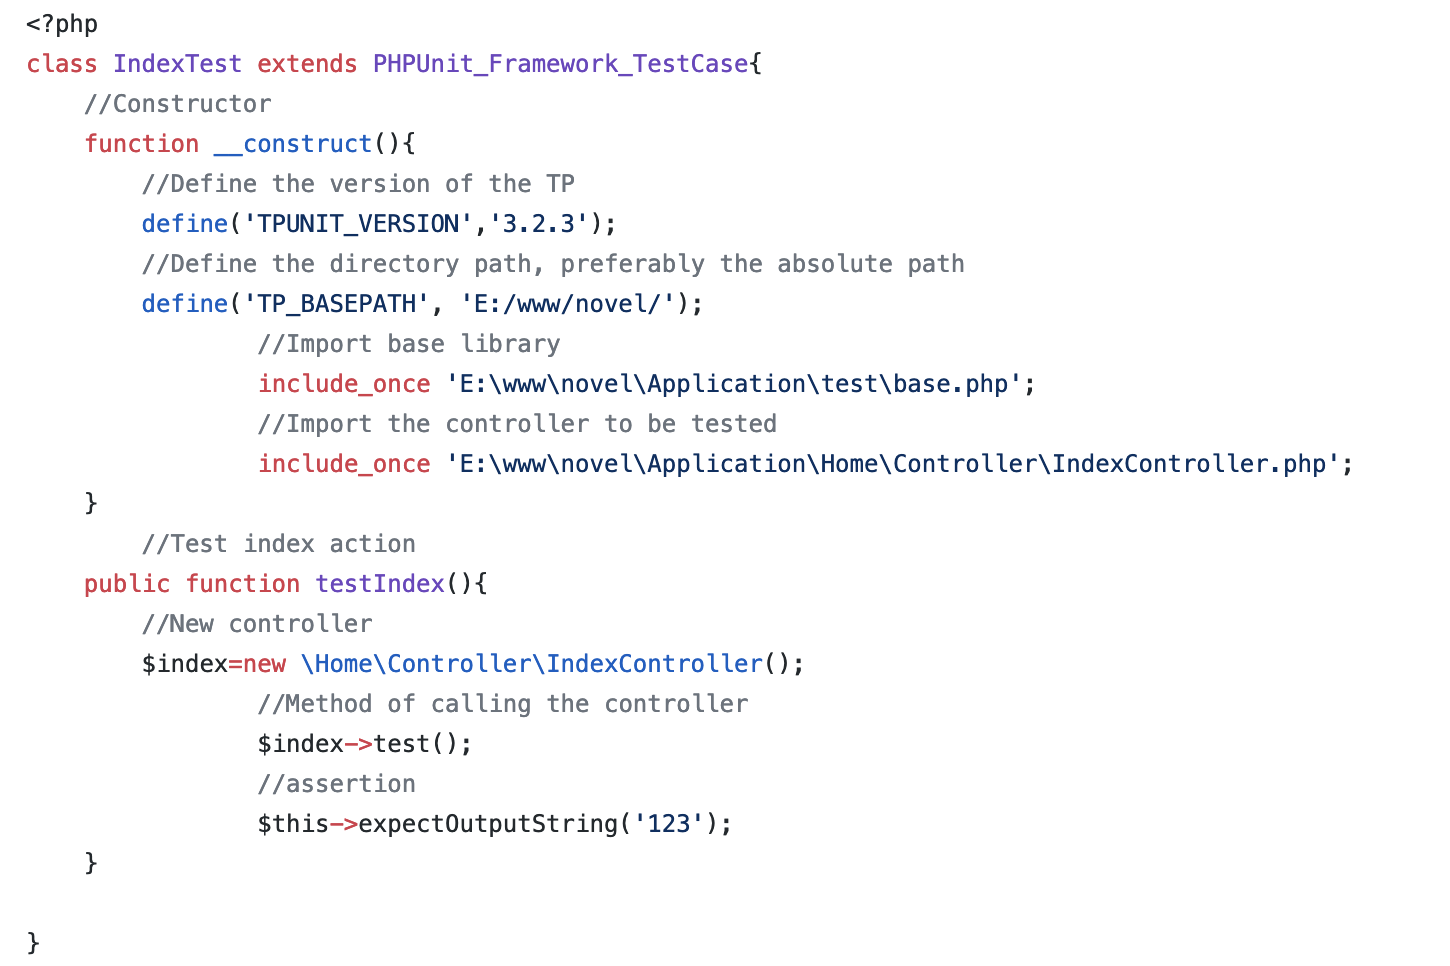
\includegraphics[width=.8\textwidth]{php.png} %图片文件的相对路径
  \caption{ThinkPHP unit testing}
  \label{php} %此处的label相当于一个图片的专属标志,目的是方便上下文的引用
 \end{figure}
    
     \item Then run phpunit for unit testing.
\end{itemize}



%关于iOS客户端的unit testing
\vspace{0.3cm}
\noindent \textbf{iOS Client Testing:}
\vspace{0.3cm}
\newline \noindent Our iOS mobile client uses the XCTest framework that comes with XCode. The word framework contains a class. All test classes inherit from this class. The name of this class is called XCTestCase. According to the regulations, the names of all test methods should start with the test and do not contain any parameters to ensure that these test methods are automatically executed when the test is run. In each test method, we call the function XCTAssert * to assert whether an operation was successful. Such automated testing of iOS development saves effort and time for developers like us.
  \begin{itemize}
      \item \textbf{iOS UI Testing}: iOS and Xcode has automated testing, click \texxxt{Command+U} in the UIText file to run the test procedure, and then use the \texxxt{red} button in the console to automatically test and generate the corresponding test code.
  \end{itemize}
